%% This is an example first chapter.  You should put chapter/appendix that you
%% write into a separate file, and add a line \include{yourfilename} to
%% main.tex, where `yourfilename.tex' is the name of the chapter/appendix file.
%% You can process specific files by typing their names in at the 
%% \files=
%% prompt when you run the file main.tex through LaTeX.
\chapter{Event Reconstruction}

The $W^{\pm}$ and $Z$ boson cross section measurements and $H \rightarrow \tau\tau$ searches rely on the precise reconstruction of the decay products. The presence of neutrinos in the leptonic $W$ decays and also in  $\tau$ decays requires an accurate reconstruction of all the detector deposits to infer the presence of the neutrinos from the momentum imbalance in the transverse plane. In addition, reconstruction of jets is important to capture the different production modes of the Higgs boson. The additional pileup interactions in the events present a challenging environment for a precise reconstruction of the events. This chapter summarizes the event reconstruction emphasizing the components relevant for the results that follow.

\section{Track reconstruction}

The goal of the track reconstruction is to estimate the position and momentum parameters of charged particles from the reconstructed hits in the inner tracking detector. Reconstructing tracks at the LHC nominal instantaneous luminosities is a computationally challenging task due to a high occupancy environment. About $1000$ charged particles transverse the inner tracking detectors at each bunch crossing. Charged particles from prior or later bunch crossings can also be present due to finite detector time resolution.  The track reconstruction starts by clustering of zero-suppressed signals in the pixel and strip detectors into hits. Each hit provides an estimate of the cluster position and the corresponding uncertainty. The CMS track reconstruction algorithm is referred to as combinational track finder (CTF)~\cite{Adam:934067,Chatrchyan:2014fea}. The CTF is an adaptation of the combinatorial Kalman filter~\cite{BILLOIR1989390,BILLOIR1990219,MANKEL1997169}, which is an extension of the Kalman filter~\cite{FRUHWIRTH1987444}, combining pattern recognition and track fitting in the same framework. 

The CTF is performed iteratively six times to determine the collection of the tracks in an event. The aim of this iterative tracking is to first find the tracks that are easiest to find (tracks with high $p_{T}$ and near the interaction region) with subsequent iterations searching for the more challenging tracks (tracks with low $p_{T}$ and displaced from the interaction region). Hits associated with tracks are removed after each iteration thereby reducing the computational complexity. Each iteration has four steps:

\begin{description}
\item[$\bullet$ Seed generation:]  Initial track candidates are found using only two or three hits in the inner part of the tracker. One has to note that the seeds are not constructed from the outermost regions of the tracker where the track density is small. The high granularity of the pixel detector ensures that the channel occupancy is lower than the channel occupancy of the outer strip layers. In addition, significant fraction of charged pions undergo inelastic interaction in the track detectors while many electrons loose significant energy due to bremsstrahlung radiation as they transverse the inner tracker. Five parameters needed to define the helical trajectory of the charged particles in the approximately uniform magnetic field. Two or three hits in combination with a constrain on the origin of the charged particle to be near the beam spot (the three dimensional profile of the luminous region of the collisions) is sufficient to extract these parameters.
\item[$\bullet$ Track finding:]  The Kalman filter algorithm is used to provide a coarse estimate of the track parameters starting from the seeds. A track candidate is built by adding hits from successive detector layers. A fast analytical propagator is used to find the hit layers. The track parameters are updated each time a new hit is found.
\item[$\bullet$ Track fitting:] The full information needed for the trajectory is only available once all the hits of the trajectory are identified. Therefore, the trajectory is once again re-fitted using a Kalman filter and smoother. A fourth-order Runge-Kutta method is used to extrapolate the trajectory between the successive hits. Material and inhomogeneous magnetic field effects are included.
\item[$\bullet$ Track selection:] Quality requirements are applied to reject fake tracks not originating from charged particles. 
\end{description}

The track reconstruction is effectively fully efficient for isolated muons with $2.5\%$ resolution in $p_{T}$ for $p_{T}$ of about $100~\GeV$~\cite{Chatrchyan:2014fea}. The longitudinal (with respect to the $z$ axis) and transverse impact parameter resolutions are $30$ $\mu$m and $10$ $\mu$m respectively. The efficiency for charged particles of $p_{T}$ greater than $0.9~\GeV$ in simulated $t\bar{t}$ events is $94\%$ ($85\%$) in the pseudorapidity region of $|\eta|<0.9$ ($0.9<|\eta|<2.4$). The main cause of the inefficiency is due to the hadrons undergoing nuclear interactions in the tracker material.   

\section{Primary vertex reconstruction}

The goal of the primary vertex reconstruction is to measure the position of each proton-proton interaction vertex in each event. The vertex reconstruction starts from the collection of the reconstructed tracks consistent with being produced near the beam spot. Additional quality requirements on the number of inner tracker layers associated to the track and the quality of the CTF fit are applied. There is no requirement on the $p_{T}$ of the tracks ensuring high vertex reconstruction efficiency.

A clustering algorithm based on the $z$ coordinates of closest approach of the tracks to the beam spot is used to resolve the vertices. The tradeoff is to be able to resolve the nearby vertices against the accidental splitting of a single vertex into more than one cluster of tracks.  A deterministic annealing (DA) algorithm~\cite{726788} is used for the clustering where the most probable vertex positions are found through a minimization of "free energy" $F$ at "temperature" $T$~\cite{Chatrchyan:2014fea}, 
\begin{equation} \label{eq:minimize}
F = -T \sum_{i}^{N_{T}} \ln \sum_{j}^{N_{V}} p_{ij} \rho_{j} \exp  \left[-\frac{1}{T}\frac{(z_{i}^{T}-z_{j}^{V})^2}{{\sigma_{i}^{z}}^2} \right],
\end{equation}
where $z_{i}^{T}$ and $\sigma_{i}^{z}$ are the $z$ coordinates of the points of the closest approach of the tracks to the $z$ and the corresponding uncertainties, $z_{j}^{V}$ are the vertex positions with vertex weights $\rho_{j}$, and $p_{ij}$ is the probability of assigning the track $i$ to the vertex $j$. The assignment of the probabilities is such that at very low temperatures every track is compatible with a single vertex while at very high temperatures all the tracks become compatible with a single vertex. The algorithm starts at a high temperature that gradually decreases ($F$ is minimized at each step) until a pre-defined minimum temperature is reached. Thereafter the temperature is further decreased to $T=1$ for the final assignment without further splitting of the vertices. 

\begin{figure}[h]
\centering
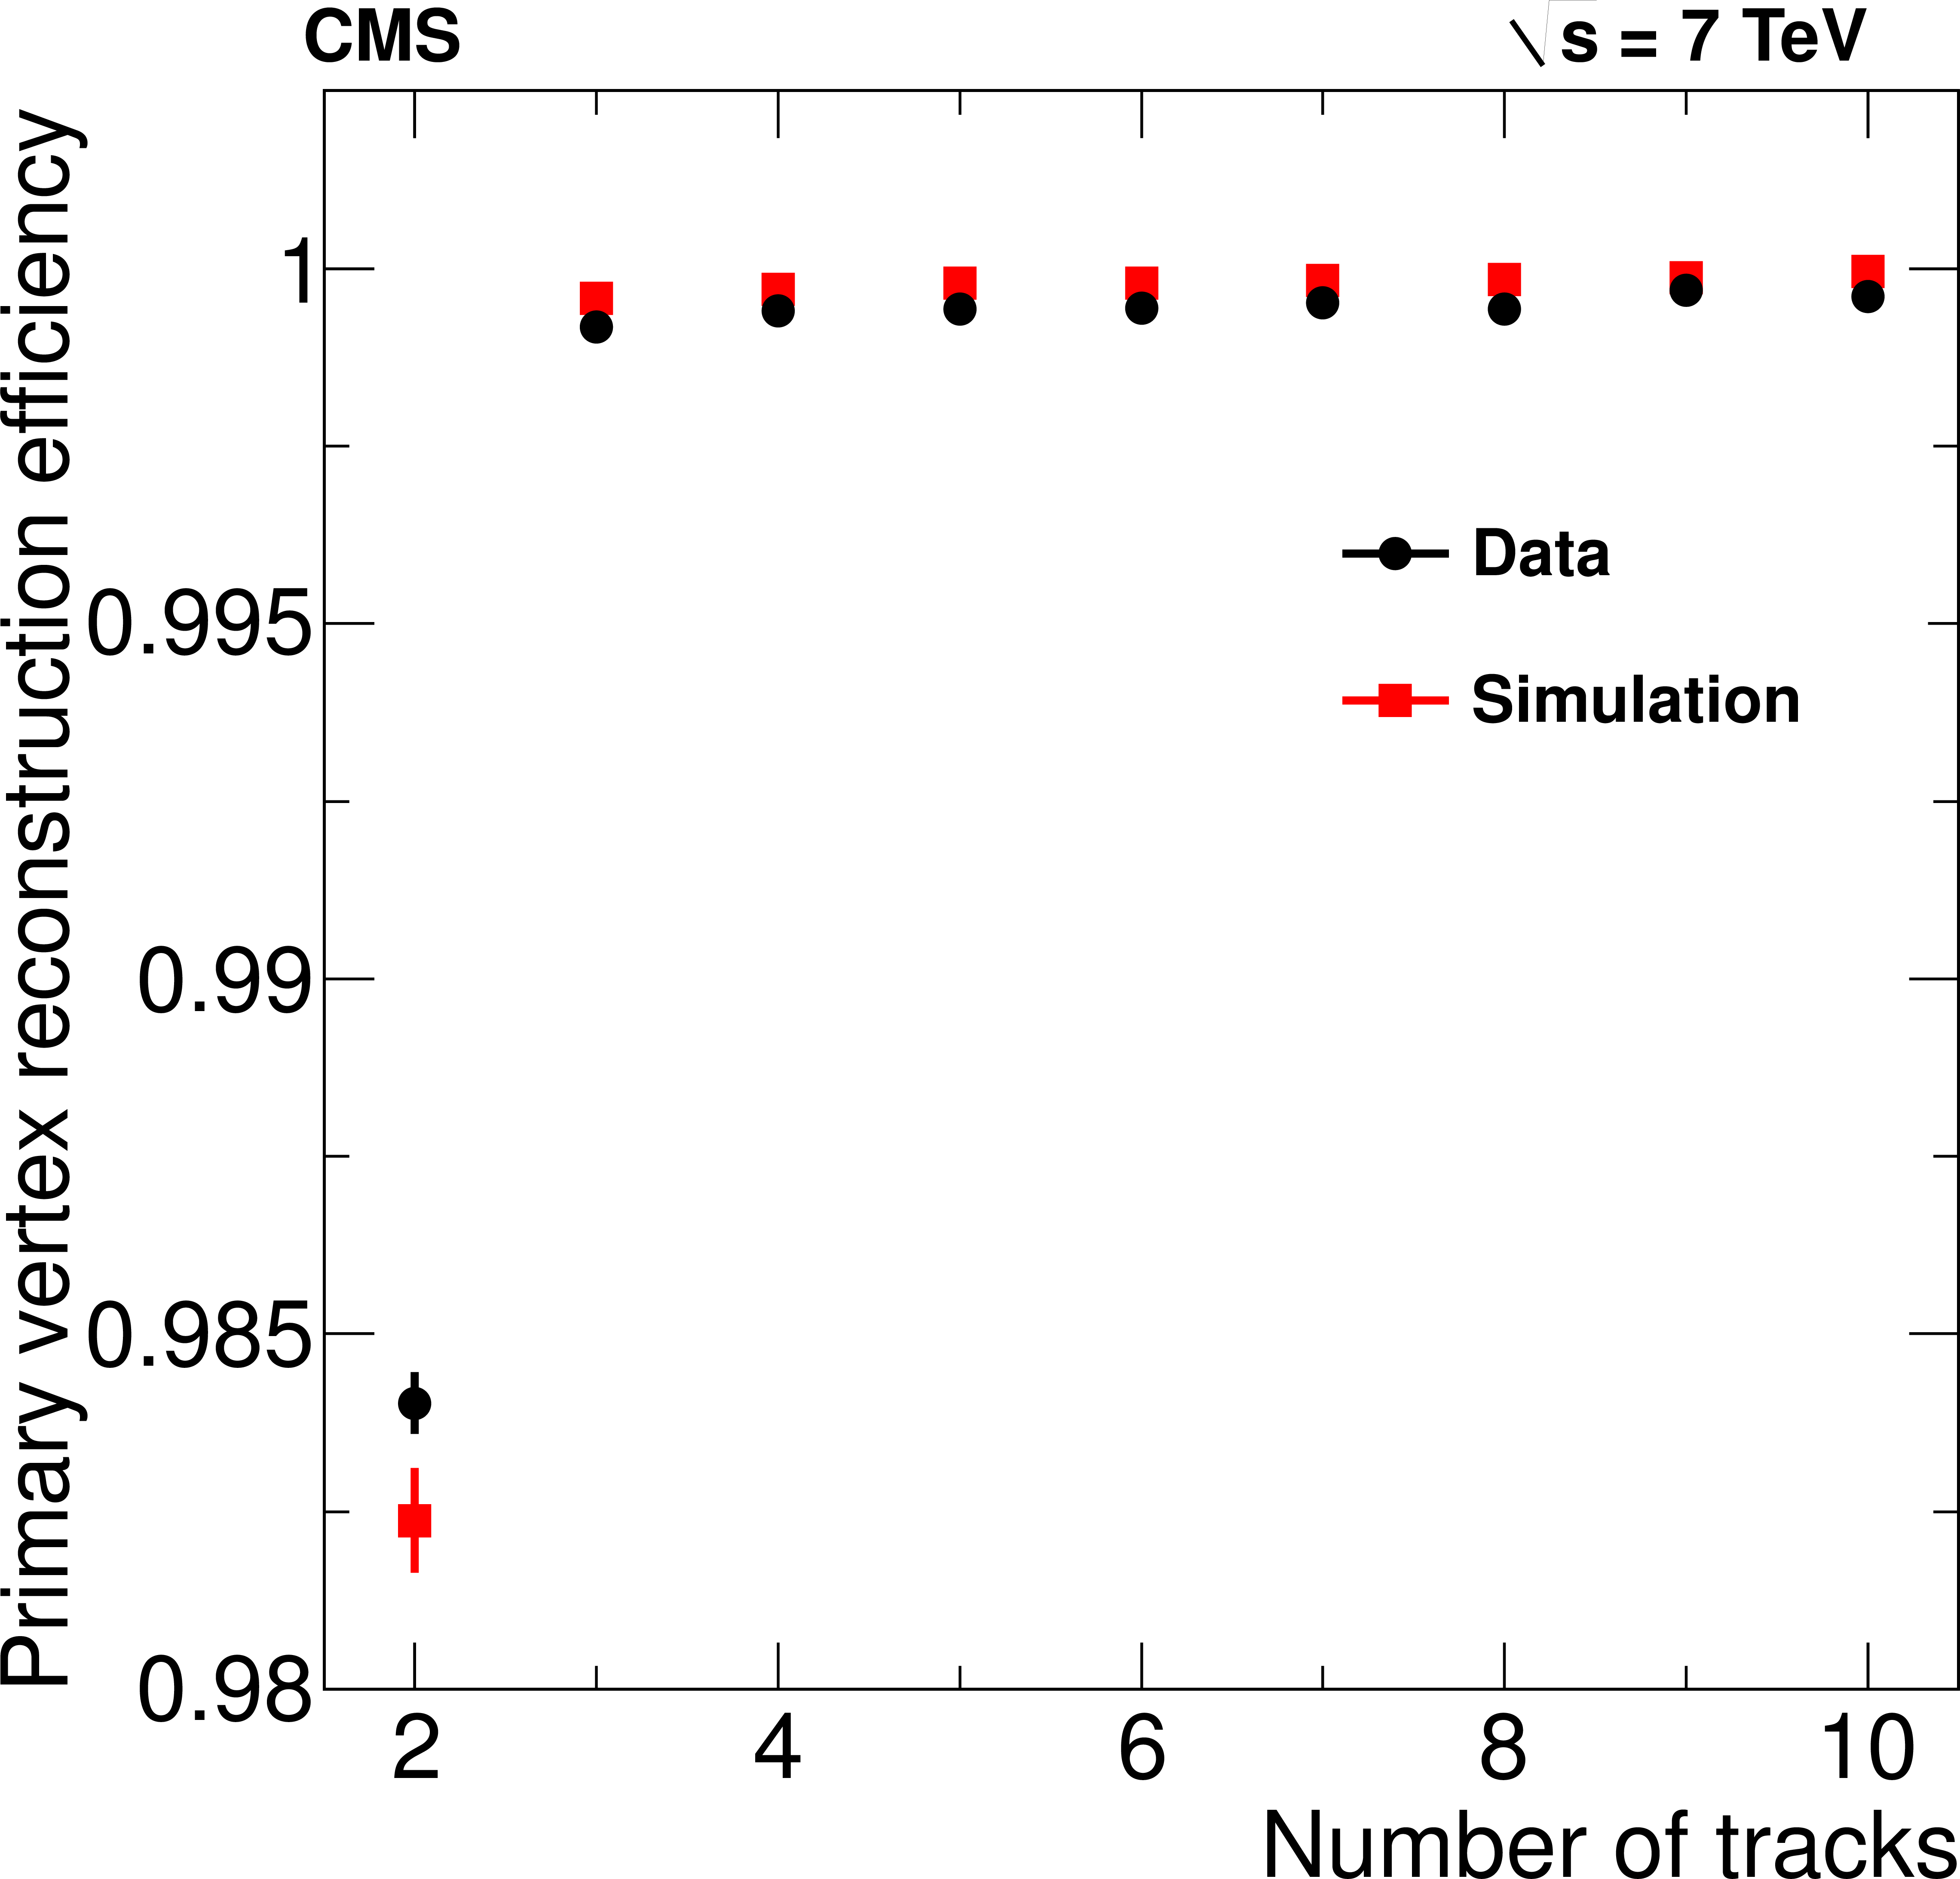
\includegraphics[width=0.49\columnwidth]{figures_chapter4/vertex_efficiency}
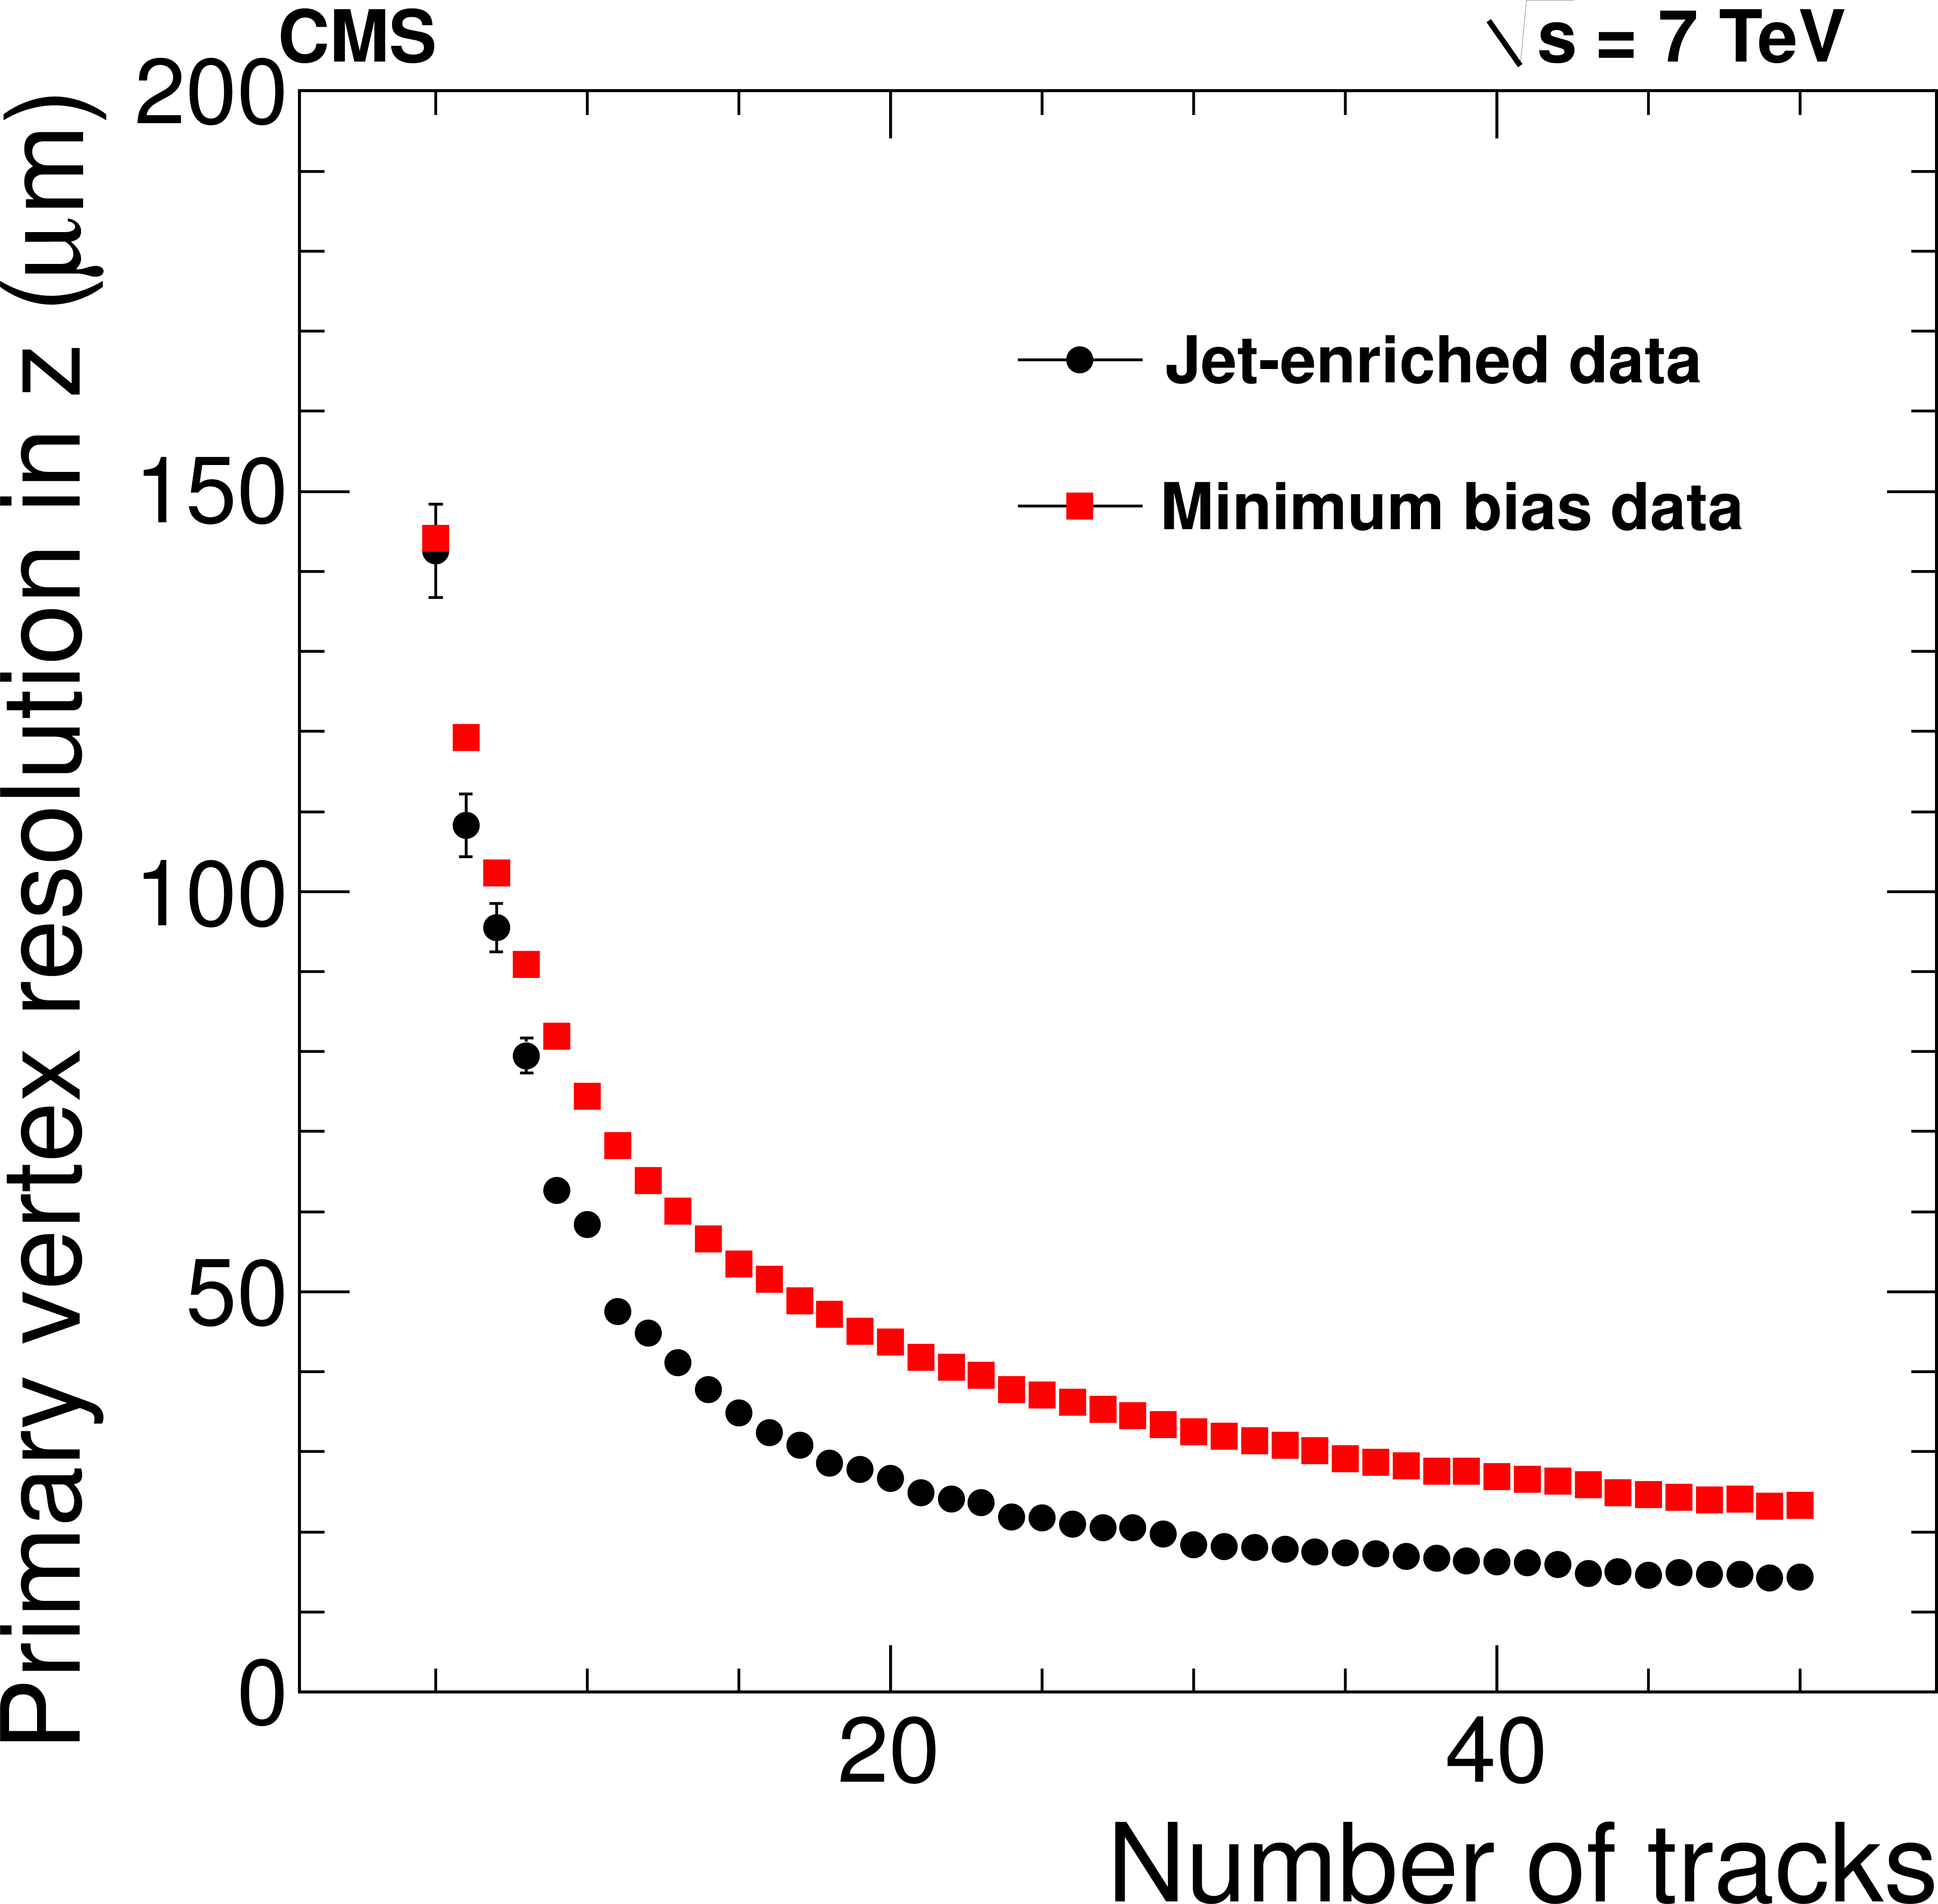
\includegraphics[width=0.49\columnwidth]{figures_chapter4/vertex_resolution}
\caption{Vertex reconstruction efficiency (left panel) as a function of the number of tracks in the vertex measured in minimum-bias data and in simulation. Vertex resolution (right panel) in the $z$ coordinate as a function of the number of tracks measured in minimum bias events (red) and jet-enriched events (black)~\cite{Chatrchyan:2014fea}.}
\label{fig:vertex}
\end{figure}

The candidate vertices determined by the DA clustering that contain at least two tracks are fitted using an adaptive vertex fitter~\cite{0954-3899-34-12-N01} to determine all the vertex parameters, including the $x$, $y$, and $z$ positions. Figure~\ref{fig:vertex} shows the vertex reconstruction efficiency (left) and vertex resolution in $z$ coordinate as a function of the number of tracks used to fit the vertex. The reconstruction efficiency is close to $100\%$ when there are more than two tracks used to reconstruct the vertex. The vertex resolution also depends on the number of tracks as well as the $p_{T}$ of the tracks. The vertex resolutions are shown for minimum bias data events (red), where loose triggers select inelastic pp collisions with as little bias as possible, and jet enriched data events, where the events are required to have a reconstructed jet with a transverse energy $E_{T}$ greater than $20~\GeV$ (black). The tracks in the jet enriched events have higher $p_{T}$ resulting in better vertex resolution. A resolution of approximately $10$ $\mu$m is achieved for high $p_{T}$ vertices with at least $50$ tracks.   

The vertex with the largest sum of the $p_{T}^2$ is defined to be the true hard-scattered pp vertex and is denoted as the primary vertex. The other vertices in the event are assumed to originate from the additional pileup interactions in the bunch crossing. Beam induced backgrounds can be rejected by applying compatibility requirements on the primary vertex with the nominal interaction point (the origin of the CMS coordinate system). The distance of the primary vertex in the $z$ direction (transverse direction) to the nominal interaction point is required to be less than $24$ cm ($2$ cm). The number of degrees of freedom of the primary vertex fit is also required to be greater than $3$.

\section{Muon Reconstruction and Identification}

Muon tracks are reconstructed not only in the CMS inner tracker but also independently in the muon system~\cite{Chatrchyan:2012xi}. The latter tracks are called standalone muon tracks. The standalone muon tracks are reconstructed from the hits in the muon chambers in a combined track fit using a Kalman filter. The "global muon" reconstruction refers to the combination and matching of the standalone muon tracks with the inner tracker tracks. A global muon track is fitted from these tracks again using a Kalman filter technique. The expected energy loss in the solenoid and support structures is taken into account in the fit. The global fit improves the momentum resolution for muons with $p_{T}$ greater than $200~\GeV$ compared to the inner tracker only resolution as demonstrated in Figure~\ref{fig:muon_resolution}.   

Another independent algorithm starts from the inner tracker and proceeds outward in the radial direction matching the hits in the muons chambers. This "tracker muon" reconstruction is more efficient for low momentum muons ($p < 5~\GeV$) compared to the global muon reconstruction as it only requires one muon segment hit in the muon chambers. The tracker muon reconstruction considers all the inner tracker tracks with $p_{T}$ greater than $0.5~\GeV$ as possible muon candidates. The average expected energy loses and multiple Coulomb scattering in the detector material are taken into account for the extrapolation to the muon system. 

\begin{figure}[h]
\centering
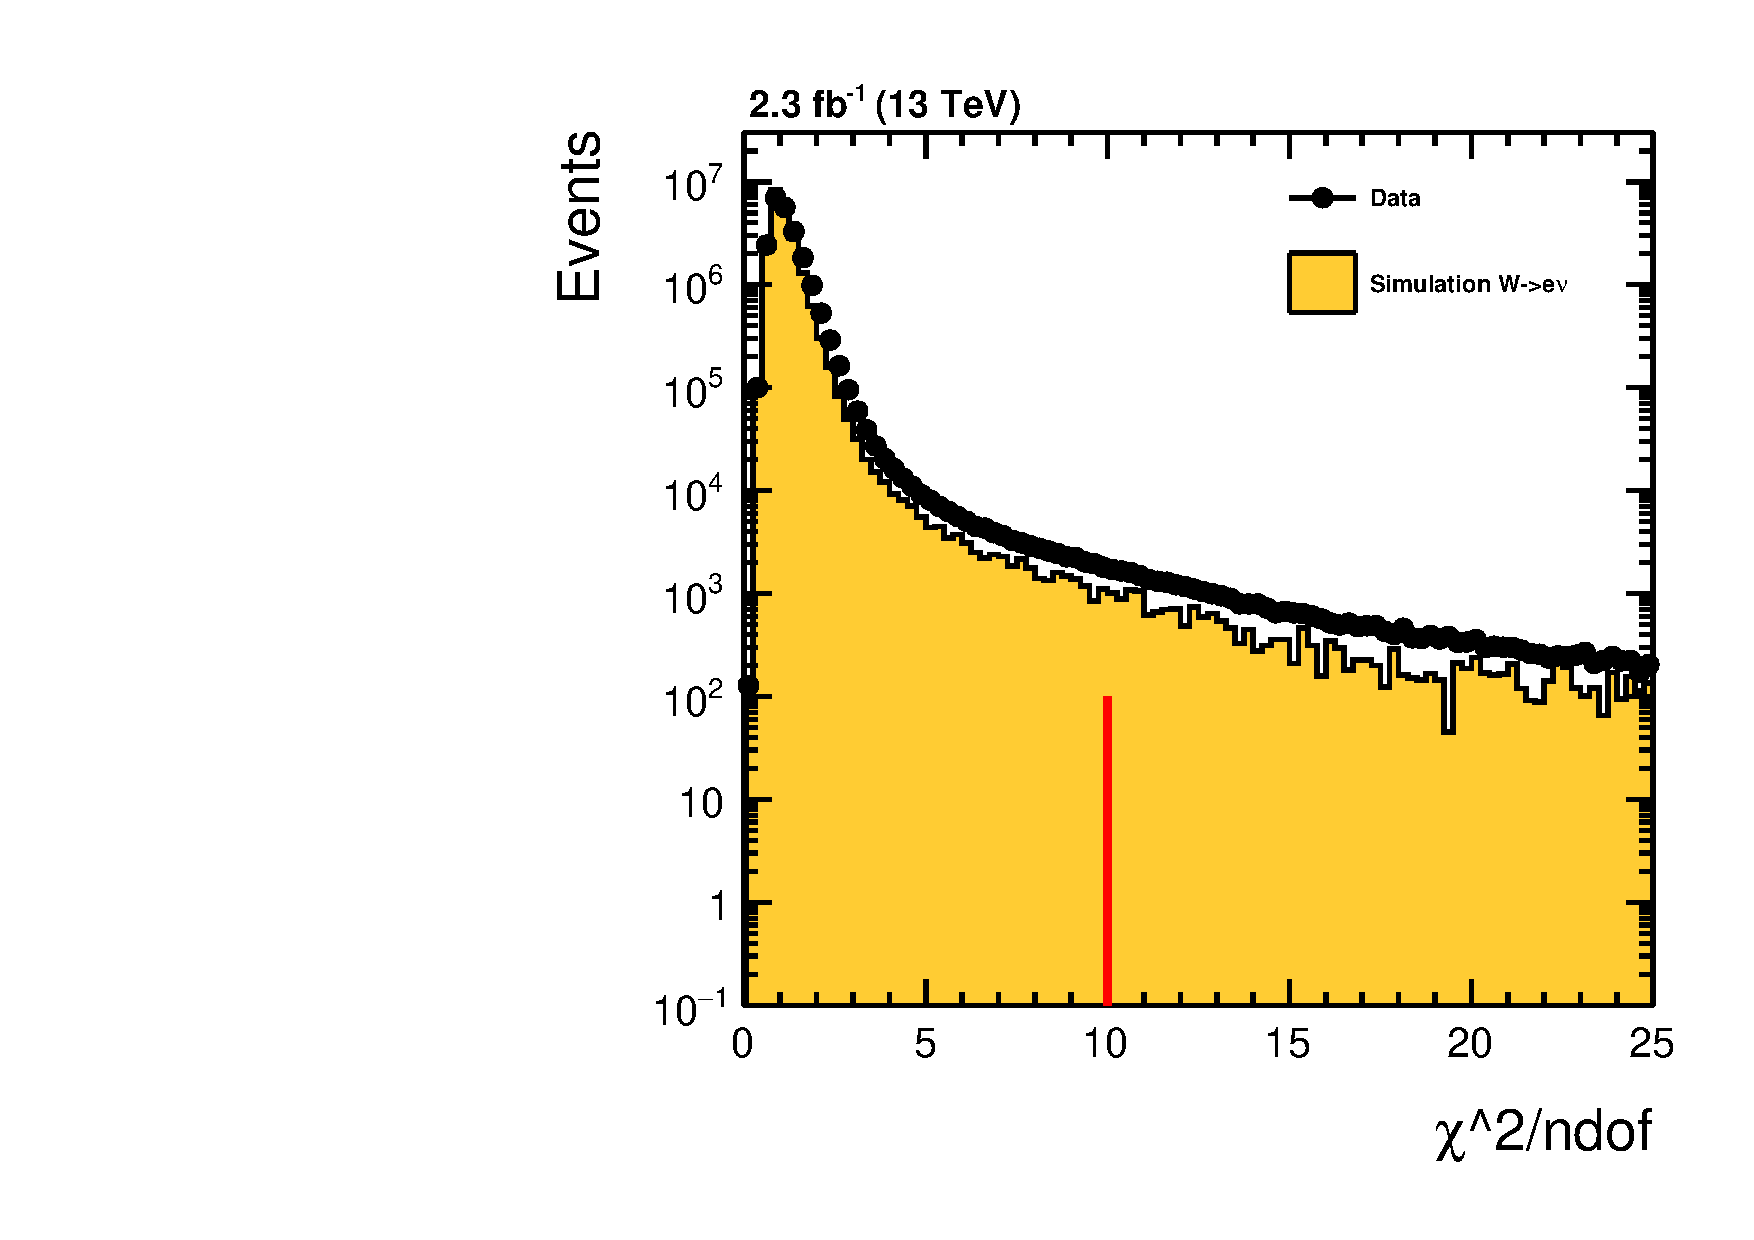
\includegraphics[width=0.49\columnwidth]{figures_chapter4/chi2_muon}
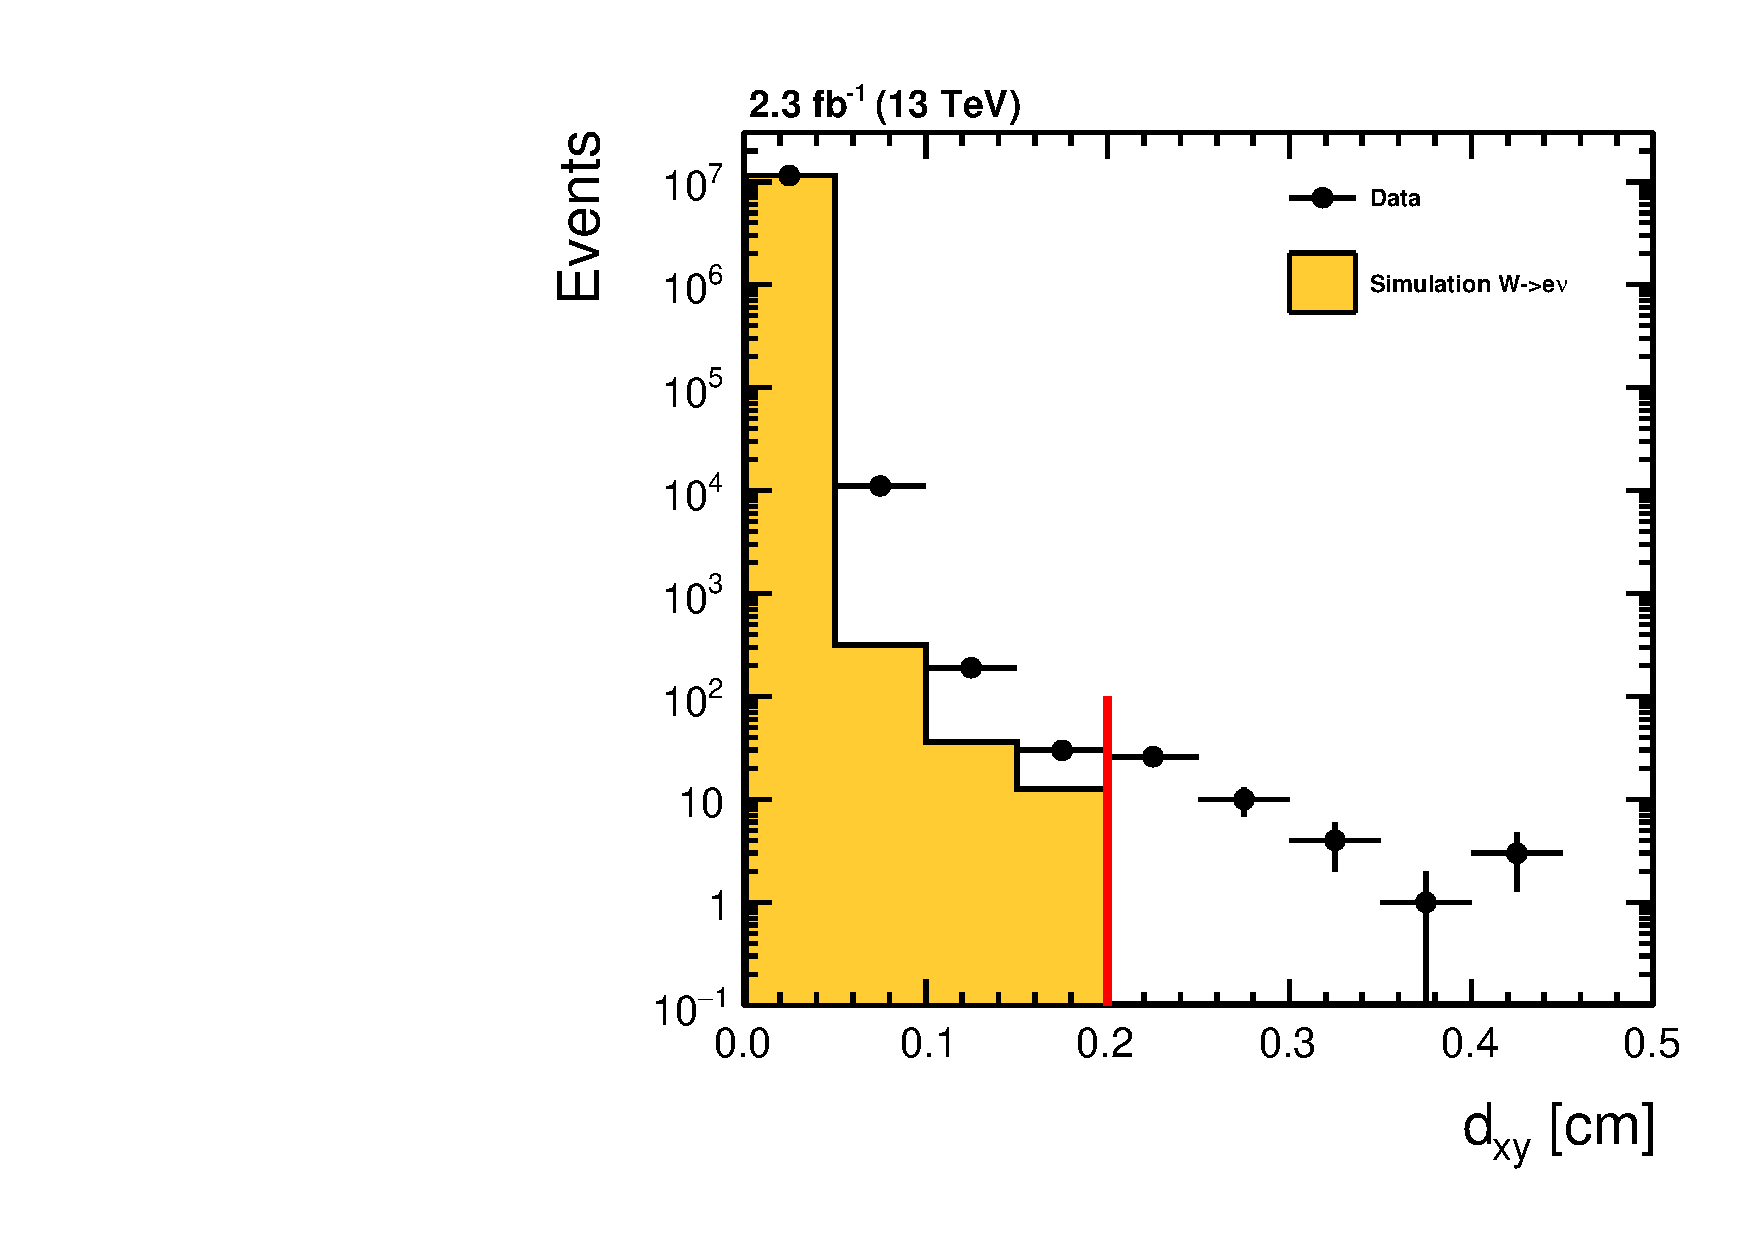
\includegraphics[width=0.49\columnwidth]{figures_chapter4/dxy_muon}
\caption{Distribution of $\chi^2$ per degree of freedom (left panel) and transverse impact parameter $d_{xy}$ (right panel) for data at $\sqrt{s}=13~\TeV$ taken during $2015$ data taking period. Simulated $W \rightarrow \mu \nu$ signal process normalized to the number of observed data evens is shown for comparison. The events satisfy all other selection requirements (including the isolation requirement to be discussed in section 3.8) are satisfied except that on the shown variable. The red line illustrates the requirement on the variable for a selection optimized for that data-taking period.}
\label{fig:muon_id}
\end{figure}

Muon candidates selected in the results are required to be a global muon. Approximately $99\%$ of the muons in the fiducial volume (the geometrical acceptance) of the muon system are identified as either a tracker or a global muon. Muon candidates identified as both a global and a tracker muon are merged into a single candidate.  Additional quality requirements are imposed to reduce miss-identified muon candidates and so called non-prompt muons. Non-prompt muons originate from in-flight decays of light hadrons and semi-leptonic decays of the heavy flavor quarks. The miss-identified muon candidates originate from the punch-through of hadron showers to the muon system. The contribution is generally small for the global muons due to the minimum number of muon segment hits requirement. 

Figure~\ref{fig:muon_id} shows the distributions of few of the muon variables used for reduction of the non-prompt and miss-identified muons. The  $\chi^2$ per degree of freedom of the global track fit is required to be less than $10$. At least one segment in the muon stations must be included in the global fit to reduce the punch-through hadrons. The muons are required to have track segments in at least two muon stations. In addition at least one hit in the pixel tracker and at least five tracking layers are required. Background originating from cosmic-ray muons transversing the CMS detector in coincidence with a pp collision is reduced by the impact parameter requirement. Figure~\ref{fig:muon_id} (right panel) shows the transverse impact parameter distribution $d_{xy}$ calculated with respect to the primary vertex. The candidates with large $d_{xy}$ originate mainly from the cosmic-ray muons. The excess of events with respect to the $W \rightarrow \mu\nu$ simulation is due to the in-flight decays of long lived particles in the QCD multi-jet background. There is also a requirement on the longitudinal impact parameter $d_{z}$ calculated with respect to the primary vertex of the event. 

\section{Electron Reconstruction and Identification}

Electrons are reconstructed by looking for a track in the inner tracker that is matched to energy deposits in the ECAL. Electron reconstruction is complicated due to bremsstrahlung radiation emitted as the electrons transverse the inner tracker detector. These bremsstrahlung photons can subsequently undergo a pair-conversion before reaching the ECAL. As a result the electron energy reaching the ECAL is significantly spread in the azimuthal direction $\phi$ due to bending of the trajectories in the CMS magnetic field. Approximately $35\%$ of electrons radiate more than $70\%$ of their initial energy before reaching the ECAL~\cite{Chatrchyan:2014fea,Baffioni:2006cd}. A dedicated clustering algorithms are used to collect the bremsstrahlung energy taking the spreading in the $\phi$ direction into account~\cite{Meschi:687345}.  The spread in the $\eta$ direction is mostly negligible except for very low $p_{T}$ (less than $5~\GeV$).    

\begin{figure}
\centering
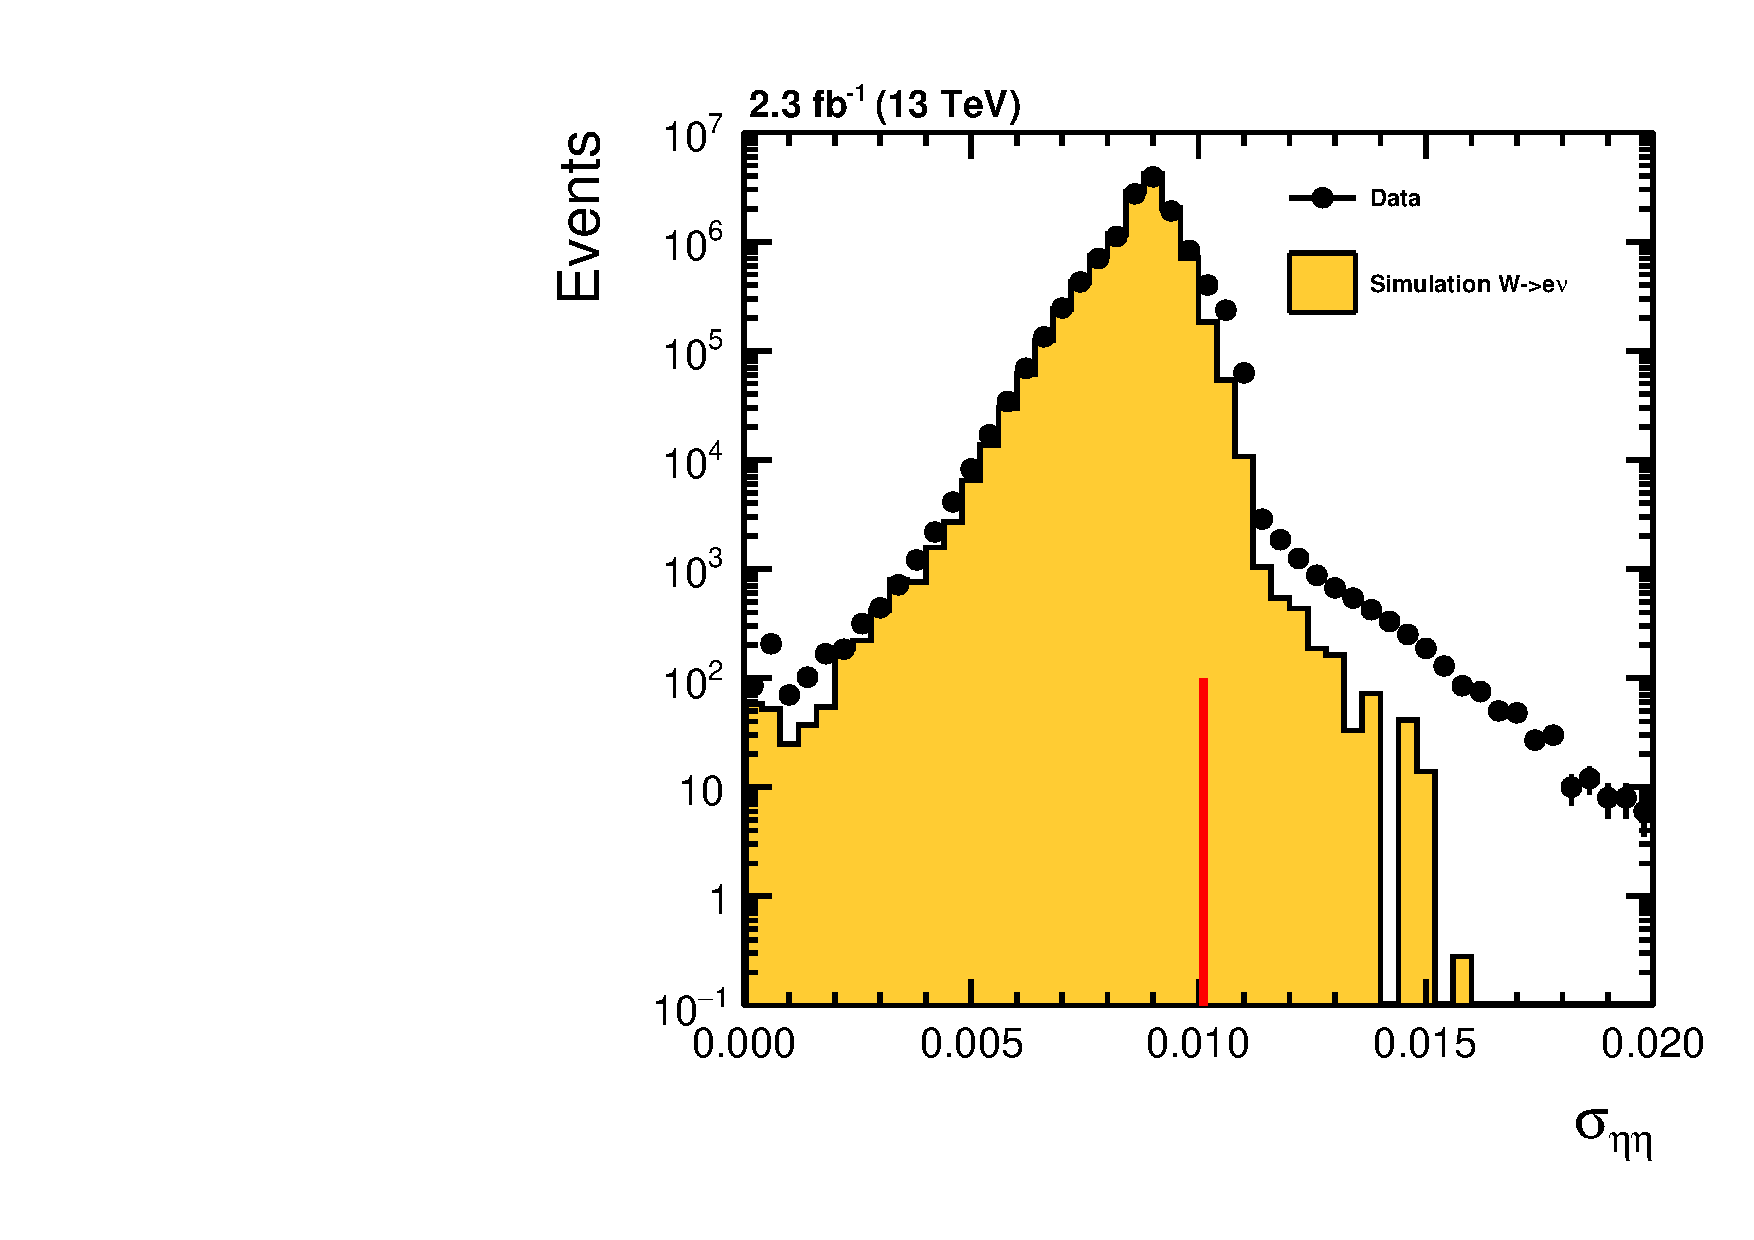
\includegraphics[width=0.45\columnwidth]{figures_chapter4/sigieie_barrel}
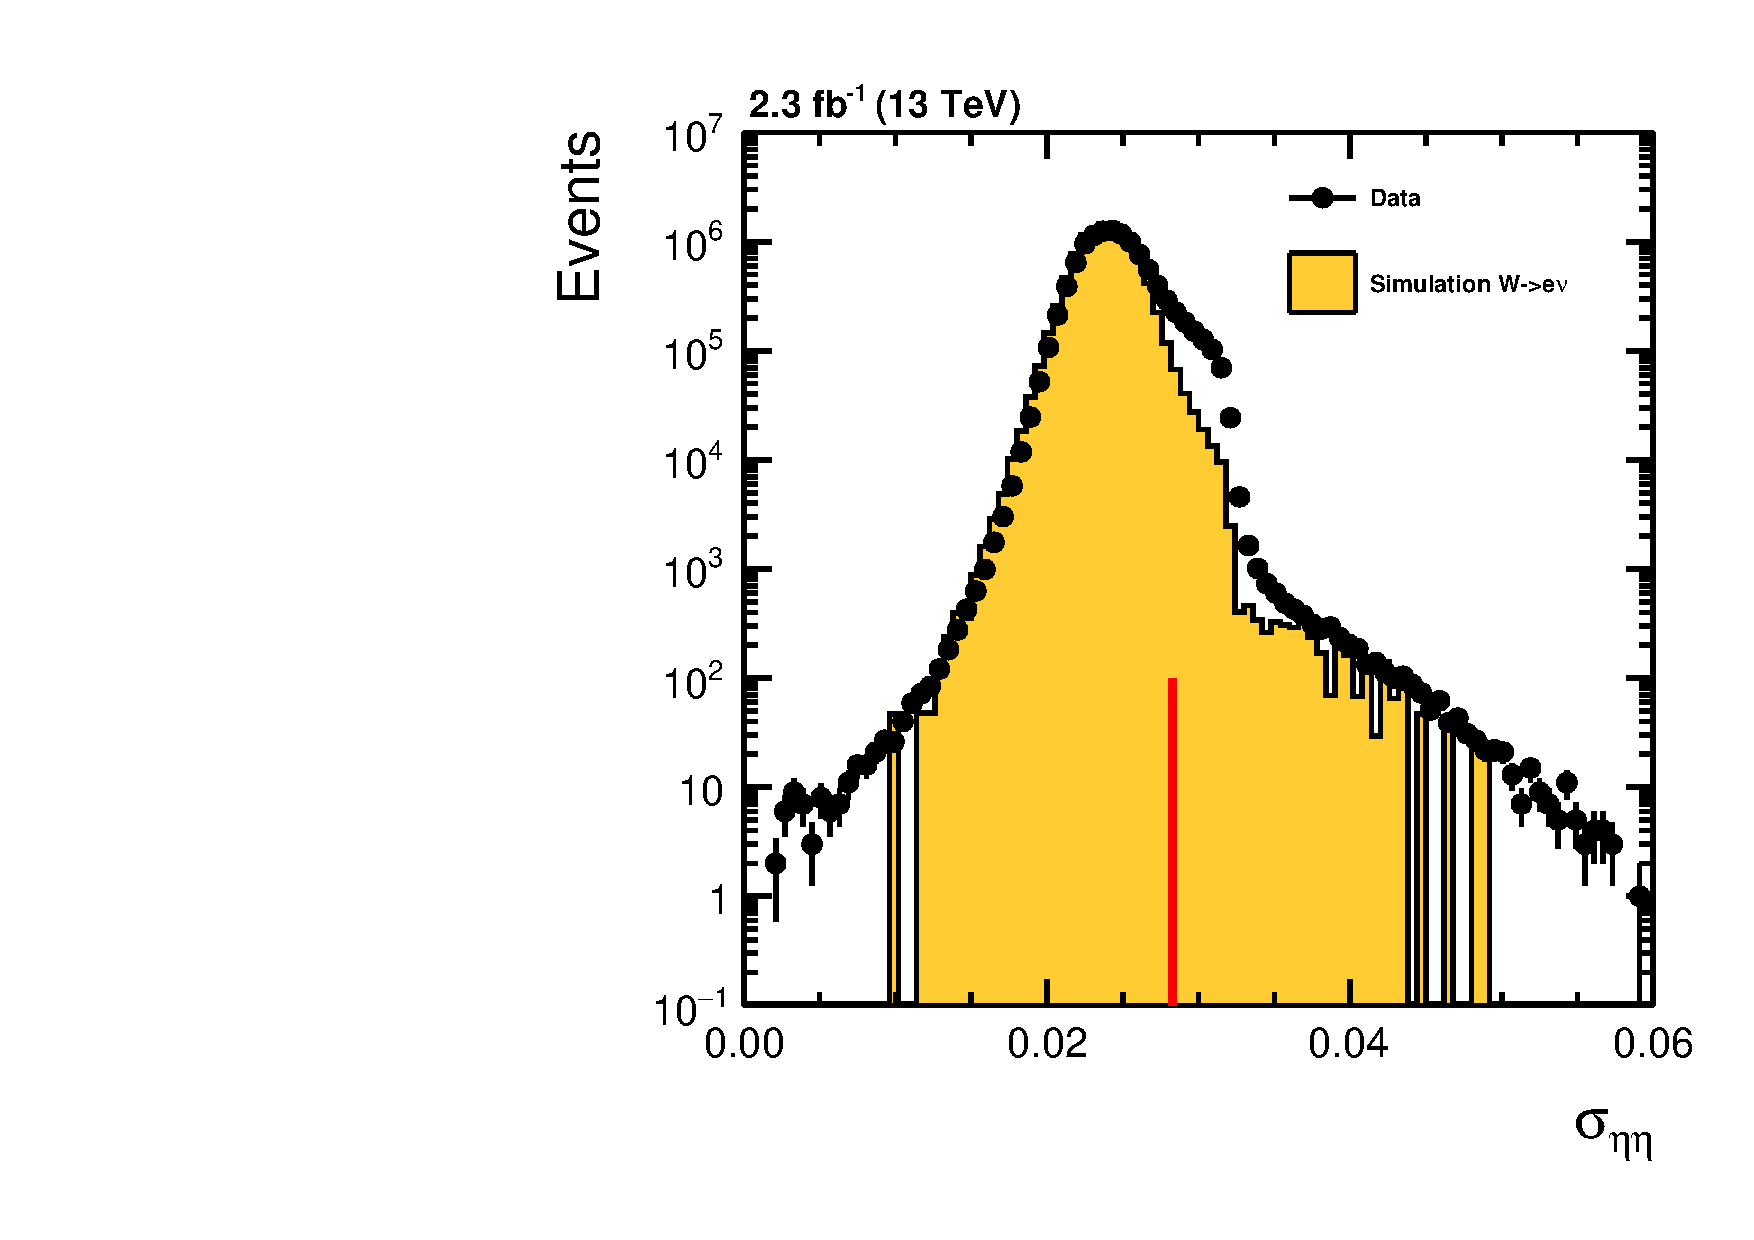
\includegraphics[width=0.45\columnwidth]{figures_chapter4/sigieie_endcap}
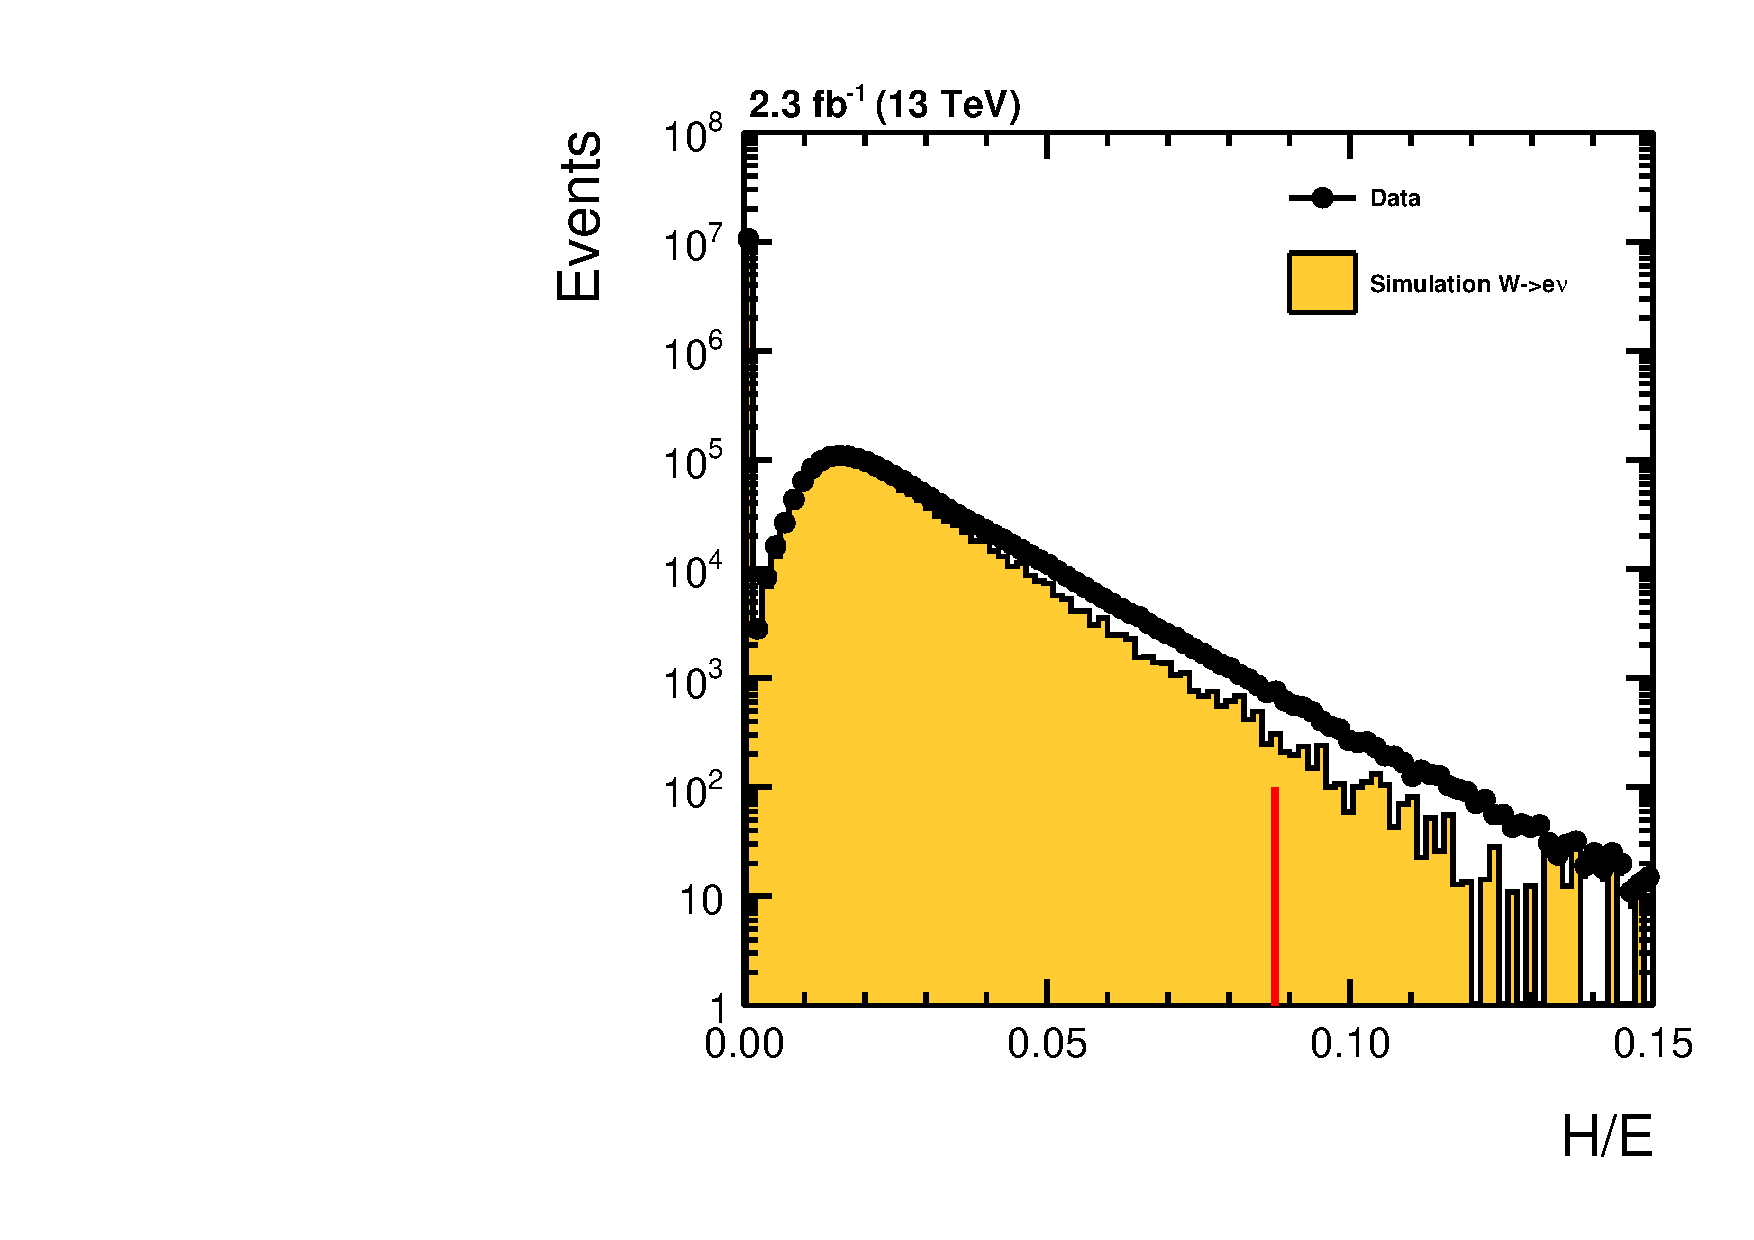
\includegraphics[width=0.45\columnwidth]{figures_chapter4/hovere_barrel}
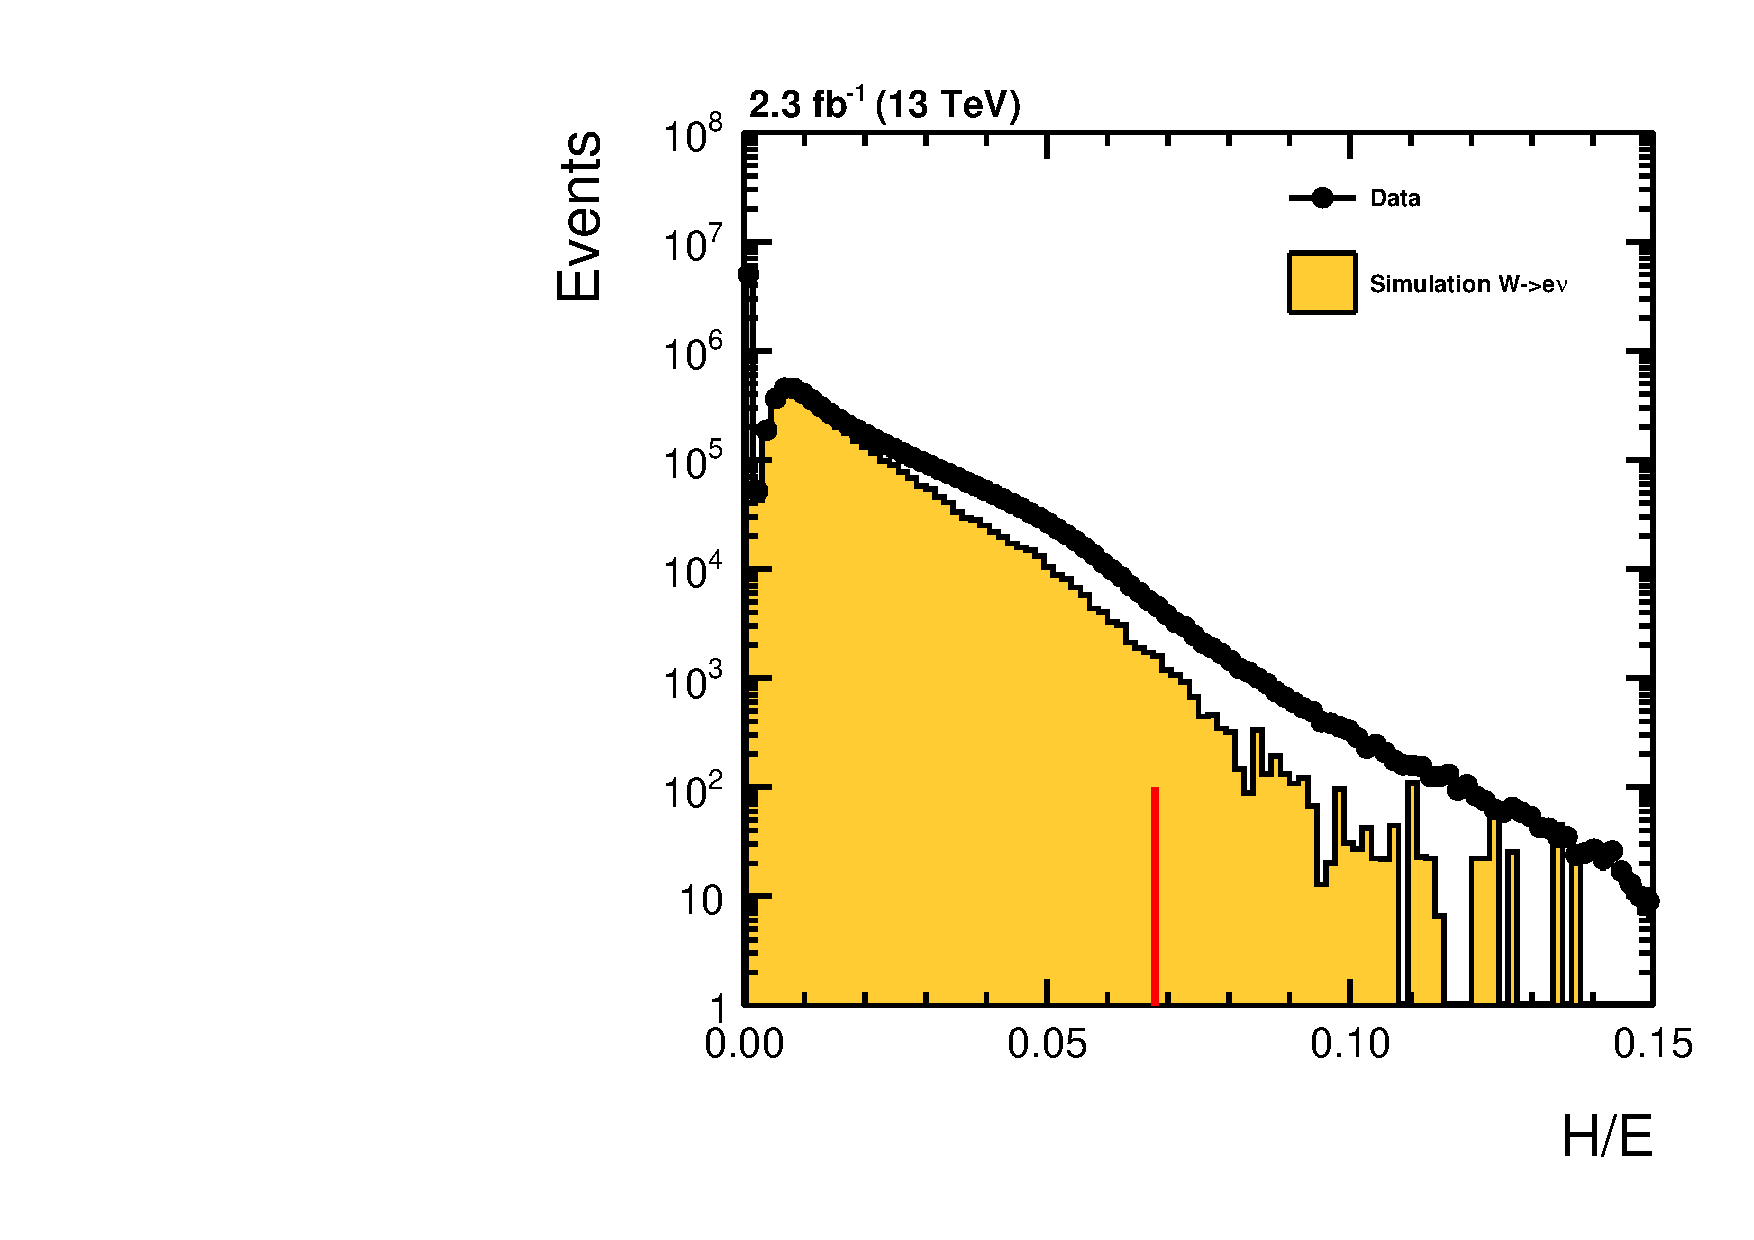
\includegraphics[width=0.45\columnwidth]{figures_chapter4/hovere_endcap}
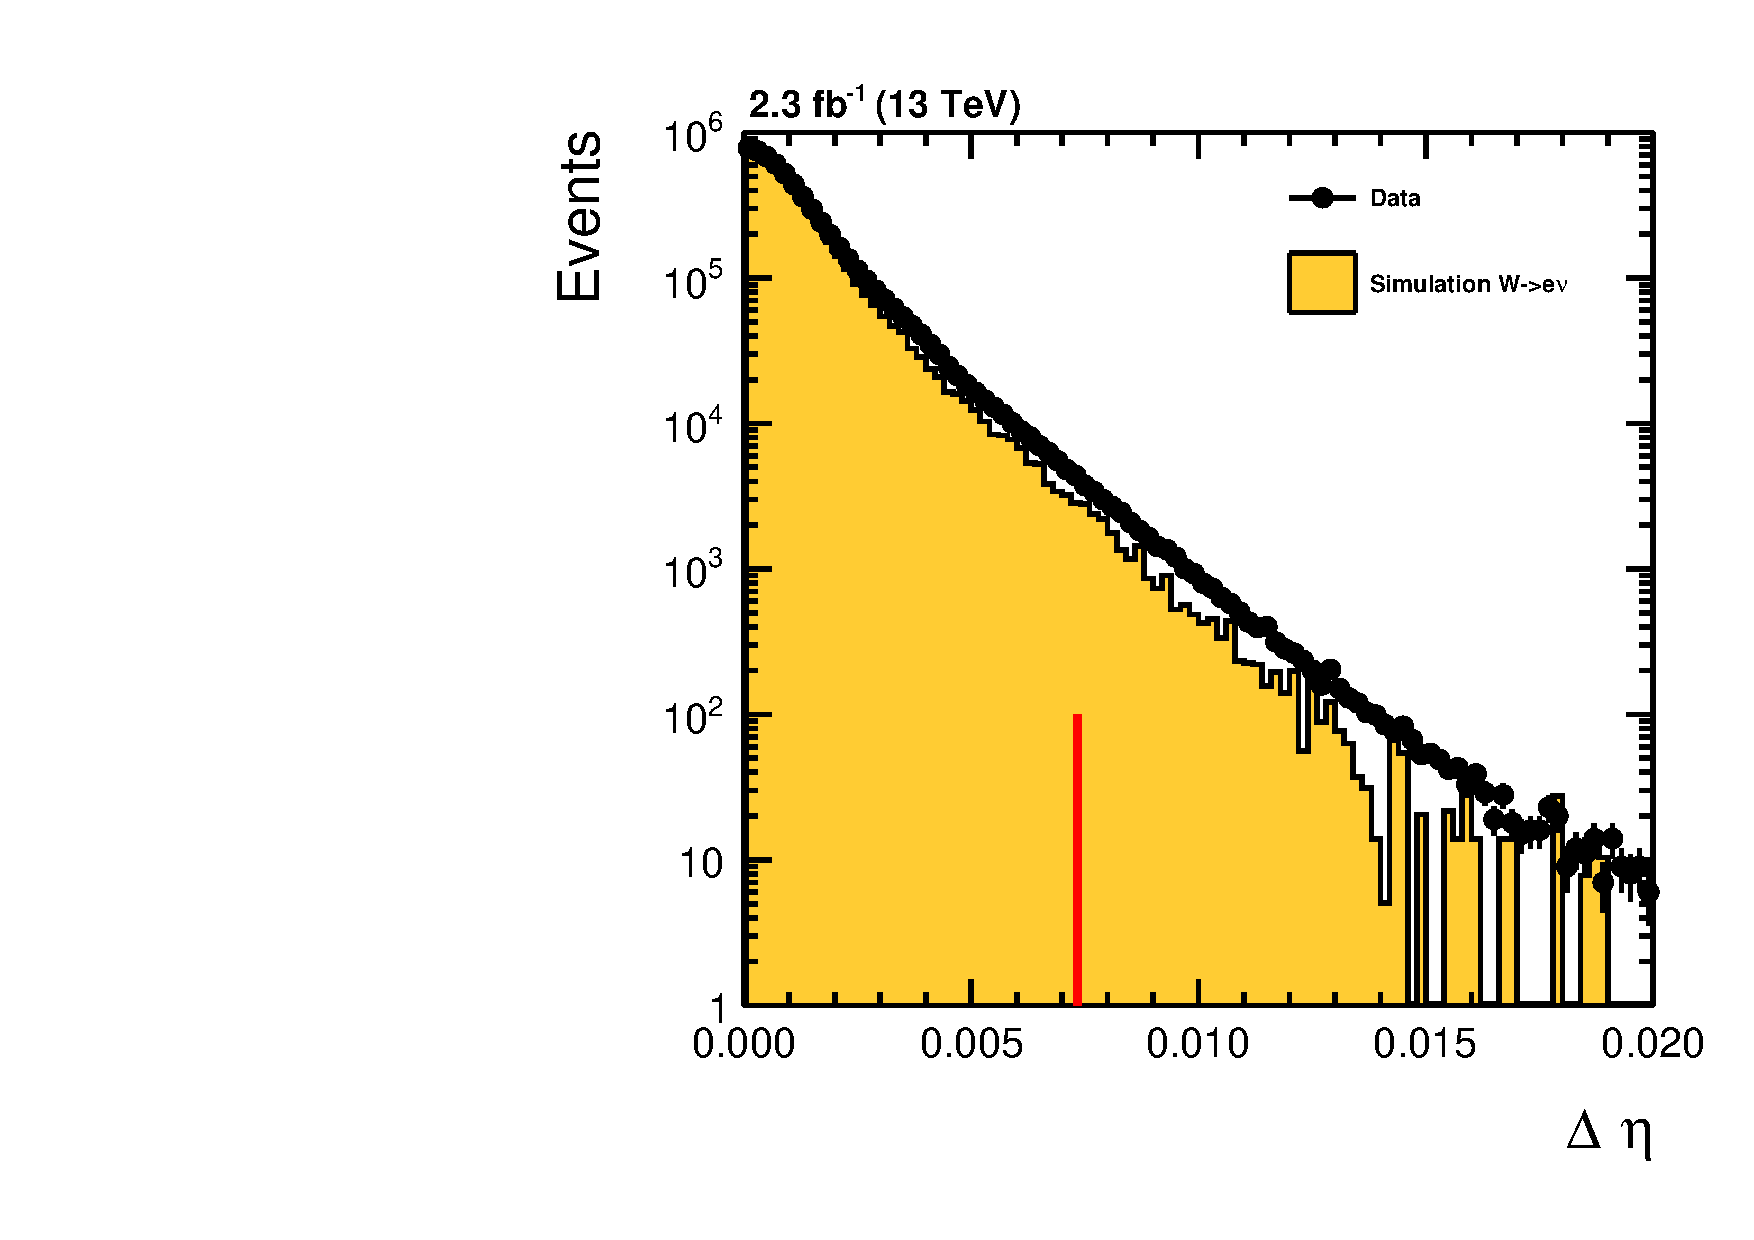
\includegraphics[width=0.45\columnwidth]{figures_chapter4/deta_barrel}
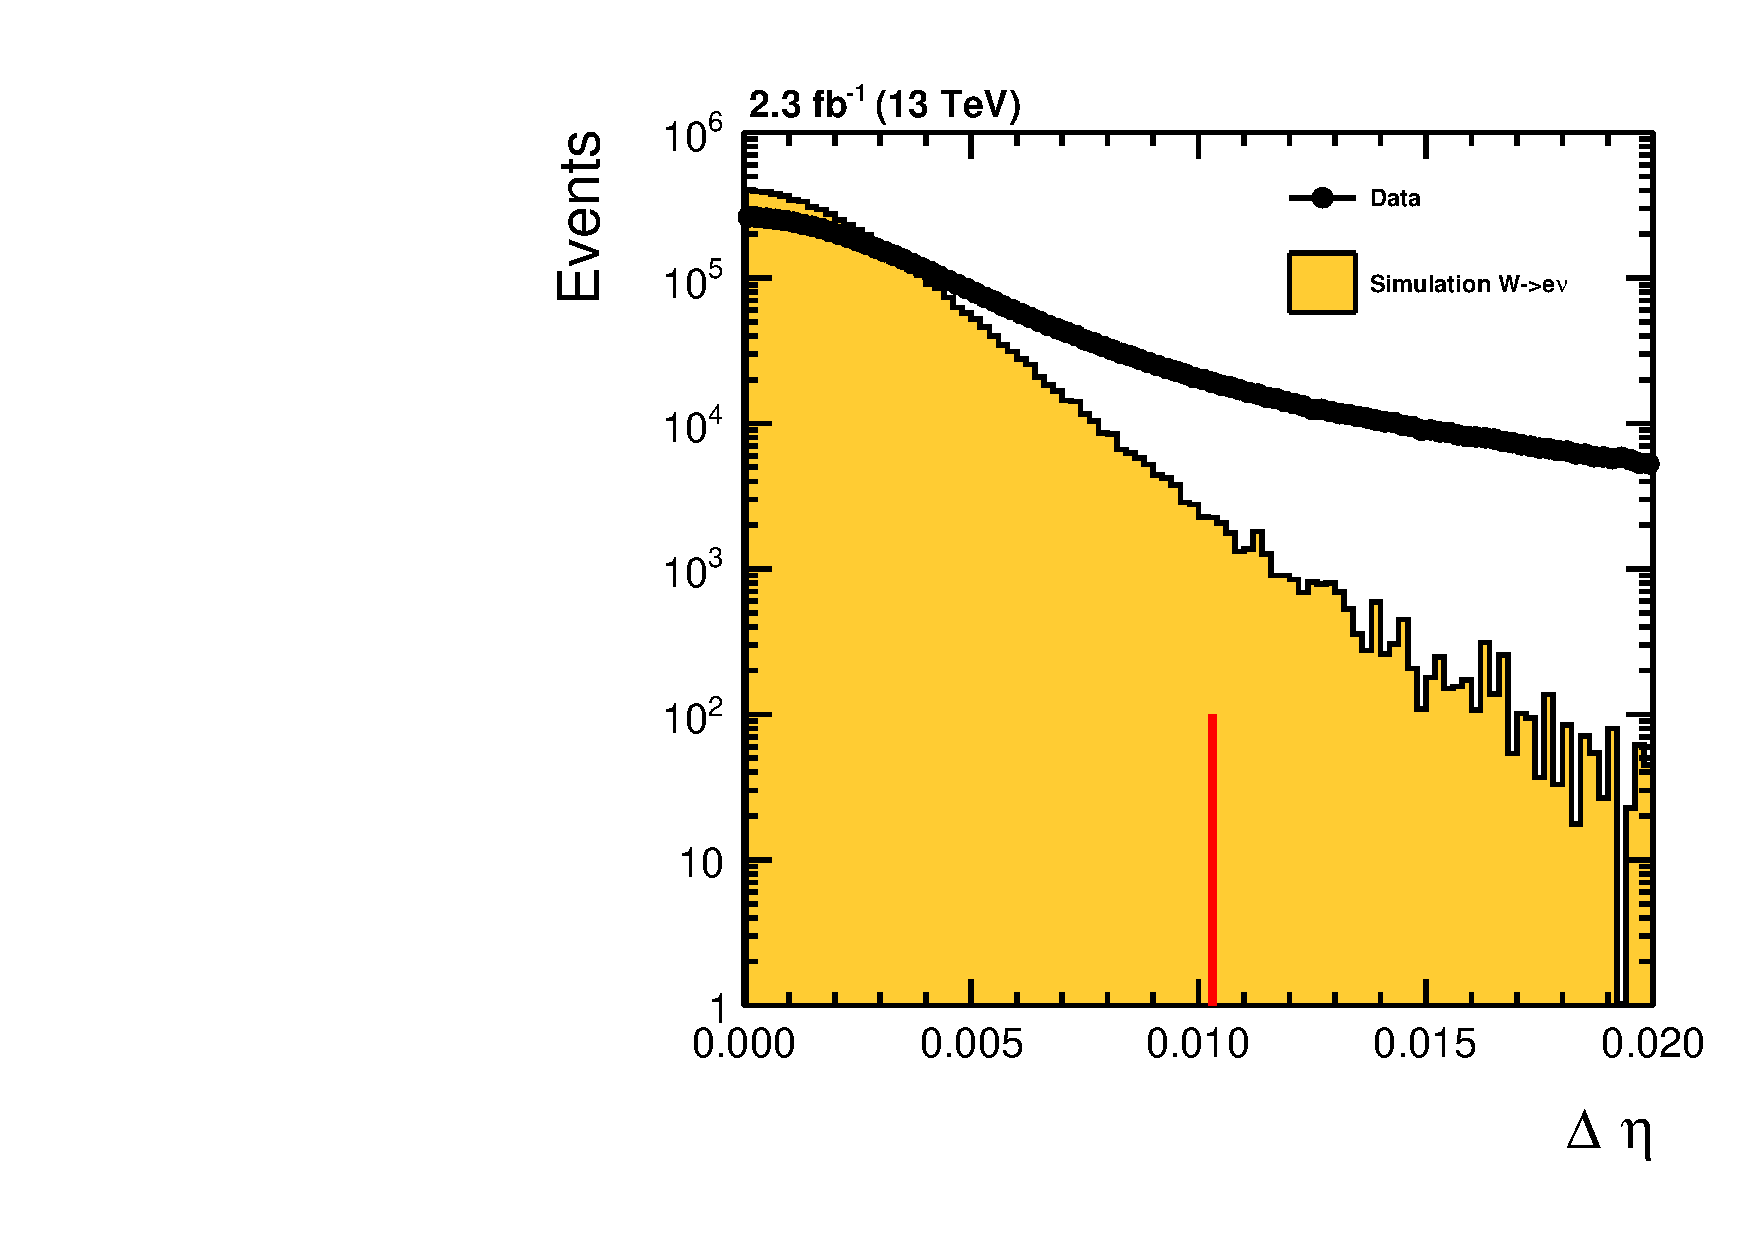
\includegraphics[width=0.45\columnwidth]{figures_chapter4/deta_endcap}
\caption{Distribution of shower shape $\sigma_{\eta \eta}$, H/E, and $\Delta \eta$ for data at $\sqrt{s}=13~\TeV$ taken during $2015$ data taking period for the barrel (left) and endcap (right). Simulated $W \rightarrow e \nu$ signal process normalized to the number of observed data evens is shown for comparison. The events satisfy all other selection requirements (including the isolation requirement to be discussed in section 3.8) are satisfied except that on the shown variable. The red line illustrates the requirement on the variable for a selection optimized for that data-taking period.}
\label{fig:ele_id}
\end{figure}

In the ECAL barrel region the energy is collected in a small $\eta$ window with an extended window in $\phi$.  An array of $5\times1$ crystals in $\eta-\phi$ are formed around a seed crystal with transverse energy $E_{T}>1~\GeV$. The arrays are extended in both $\phi$ directions centered at the seed crystals up to $\Delta \phi$ of radius of $0.3$. The arrays with $E_{T}>0.1~\GeV$ are grouped to form a supercluster. In the ECAL endcap the supercluster is seeded by a $5\times5$ cluster in $\eta-\phi$ centered at the seed crystal. The supercluster energy corresponds to the sum of the energies of its clusters. 

Inner tracker seeds compatible with a reconstructed supercluster are searched in the pixel tracker (also in TEC to improve the efficiency). Electrons that suffer a small amount of bremsstrahlung radiation loss can be identified by extrapolating a standard reconstructed track to the ECAL and checking if it passes close to an ECAL cluster. On the other hand a poor $\chi^2$ or few associated hits in the reconstructed tracks may come from an electron that suffered a significant bremsstrahlung energy loss. A modified version of the Kalman filter is used to perform the final fit of the track parameters as the Kalman filter is only optimal for Gaussian uncertainties whereas the bremsstrahlung energy loss is modeled by Bethe-Heitler.  A gaussian approximation to the Bethe-Heitler model is crude and therefore a Gaussian-Sum filter (GSF)~\cite{Adam:815410} method is employed that approximates the Bethe-Heitler energy loss by a sum of Gaussian functions.The final electron momentum is derived from a weighted mean of the inner tracker measurements and the supercluster energy. 

There are few sources of electron backgrounds. An overlapping charged and neutral pions inside a hadronic jet or a charged pion showering early in the ECAL can be miss-identified as an electrons. Figure~\ref{fig:ele_id} shows the distributions of few of the electron identification variables used for reduction of these background processes:
 
\begin{description}
\item[$\bullet$]  $\sigma_{\eta\eta}$ is the energy weighted $\eta$ width of the cluster. As can be seen it is small for genuine electrons.  
\item[$\bullet$]  H/E is the ratio of the energy deposited in the HCAL to the electromagnetic energy near the seed cluster.
\item[$\bullet$]  $\frac{1}{E}-\frac{1}{p}$ quantifies the energy and momentum compatibility measured in the ECAL and inner tracker respectively.
\item[$\bullet$] $\Delta \eta$ and $\Delta \phi$ are the separations between the supercluster and track directions evaluated at the primary vertex in the $\eta$ and $\phi$ directions respectively.    
\end{description}

The conversion of a photon into an electron-positron pair is another source of background. Electron candidates with missing hits in the innermost layers of the inner tracker indicate a photon conversion. An identification of a vertex with a pair of tracks with no hits in the tracker layers between the vertex and the interaction point is also used to further suppress this background. 

\section{Jet Reconstruction}

Quarks and gluons produced at the LHC fragment and hadronize nearly immediately to a collimated spray of hadrons known as jets. Jets may originate from a $2 \rightarrow 2$ scattering of the partons inside the colliding protons, decay of q heavy object, such as a top quark or a Higgs boson, and emission of gluons off some other partons in the event. Measuring the jet energy and direction provides information of the original parton. A detailed review of jet finding algorithms, a set of rules for grouping the hadrons into jets, at hadron colliders can be found in~\cite{Salam:2009jx}. So called sequential recombination jet algorithms are used at CMS as implemented in the FastJet package~\cite{Cacciari:2011ma}.  The usual approach of these algorithms is to introduce two distance measures $d_{ij}$ and $d_{iB}$ defined as:
\begin{eqnarray} \label{eq:jet_find}
d_{ij} = min(p_{ti}^{2p},p_{tj}^{2p})\frac{\Delta_{ij}^2}{R^2}, \\
d_{iB} = p_{ti}^{2p},
\end{eqnarray}
where $\Delta_{ij}^2 = (y_{i}-y_{j})^2 + (\phi_{i} -\phi_{j})^2$ and $k_{ti}$, $y_{i}$, and $\phi_{i}$ are the transverse momentum, rapidity, and azimuth of object $i$ in the event. $R$ is the distance parameter and $p$ is the power of the energy scale. From the above definitions it is seen that $d_{ij}$ and $d_{iB}$ are invariant under a boost along the beam direction. The algorithm proceeds to identify the smallest distance measures in the events. If $d_{ij}$ is the smallest for a given pair of objects, then the two objects are combined into a single object by adding the momenta of the $i$ and $j$ objects. If $d_{iB}$ is the smallest distance then the object $i$ is denoted as a jet and removed from further consideration in the algorithm. The algorithm continues until there are no objects remaining in the event. The anti-$k_{t}$ algorithm~\cite{Cacciari:2008gp} with $p=-1$ is used for the results shown here. A distance parameter of $R=0.5$ or $R=0.4$ is used. The anti-${k_{t}}$ algorithm grows outward from hard "seeds" resulting in a cone-like jets in $\eta-\phi$. The resulting jet boundaries are resilient with respect to soft radiation while the algorithm is infra-red and collinear safe.  


\subsection{Jet Energy Scale}

Jet energy needs to be calibrated to obtain a more accurate estimate of the original parton energy. Corrections are needed to account for the additional energy due to pileup, non-uniformities in the detector response, and detector noise. The effect of additional energy due to pileup and detector noise is corrected on per-jet basis for each event using the median energy density $\rho$ and the jet area~\cite{Cacciari:2007fd}. Pseudorapidity and jet transverse momentum dependent corrections are derived in simulated events with and without pileup overlay. "Zero-bias" triggered events (from randomly selected non-empty LHC bunch crossings) are used to correct for the residual differences between data and detector simulation.  The average jet energy scale is calibrated using the MC truth in simulation~\cite{1748-0221-6-11-P11002,Khachatryan:2016kdb}. Corrections are then applied to to account for residual differences  between the detector simulation and data using the transverse momentum balancing in di-jet, $\gamma$-jet, and $Z$-jet events. The di-jet $p_{T}$ balancing method is used to correct the relative scale using the barrel region $|\eta|<1.3$ as a reference. The absolute scale is corrected using $\gamma$-jet and $Z$-jet events exploiting the excellent $p_{T}$ resolution of photons and leptons. 

\begin{figure}[h]
\centering
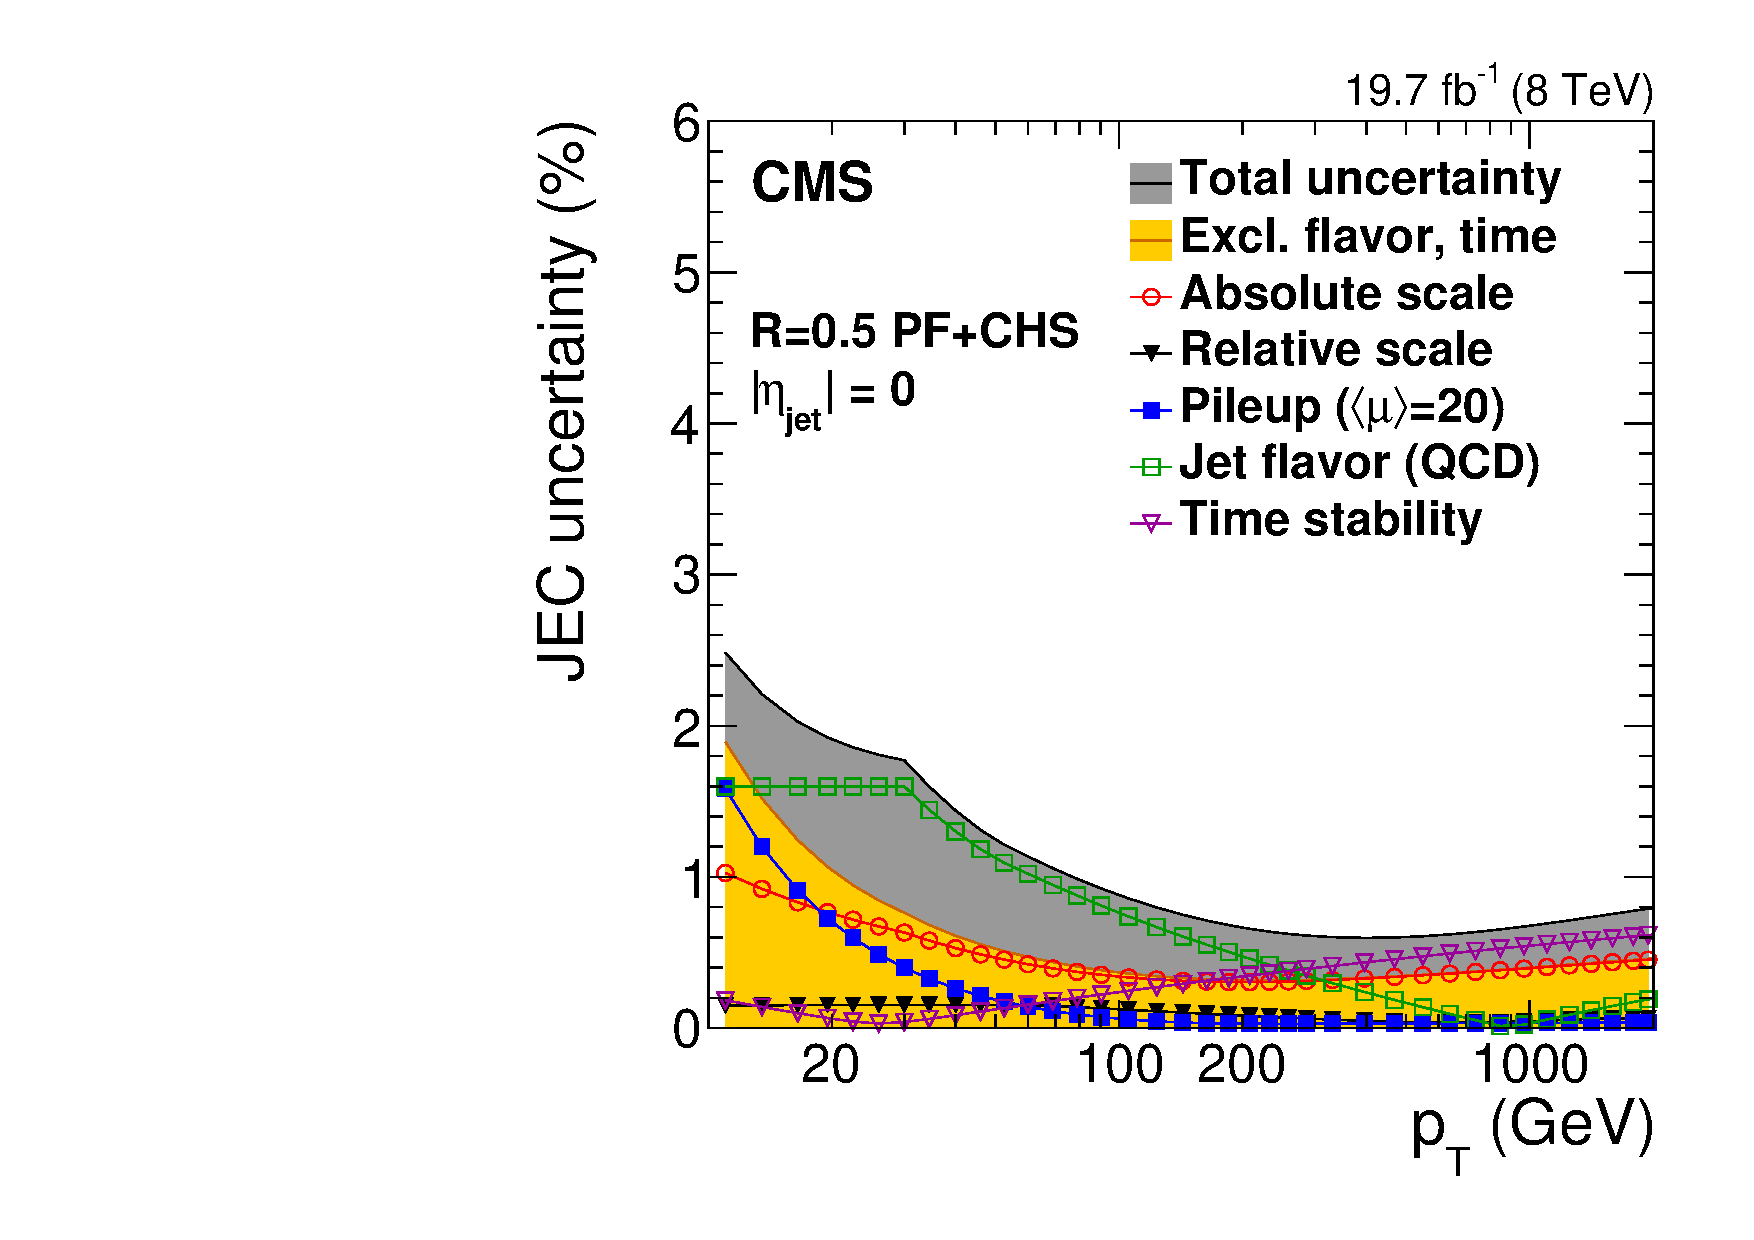
\includegraphics[width=0.49\columnwidth]{figures_chapter4/jec_unc}
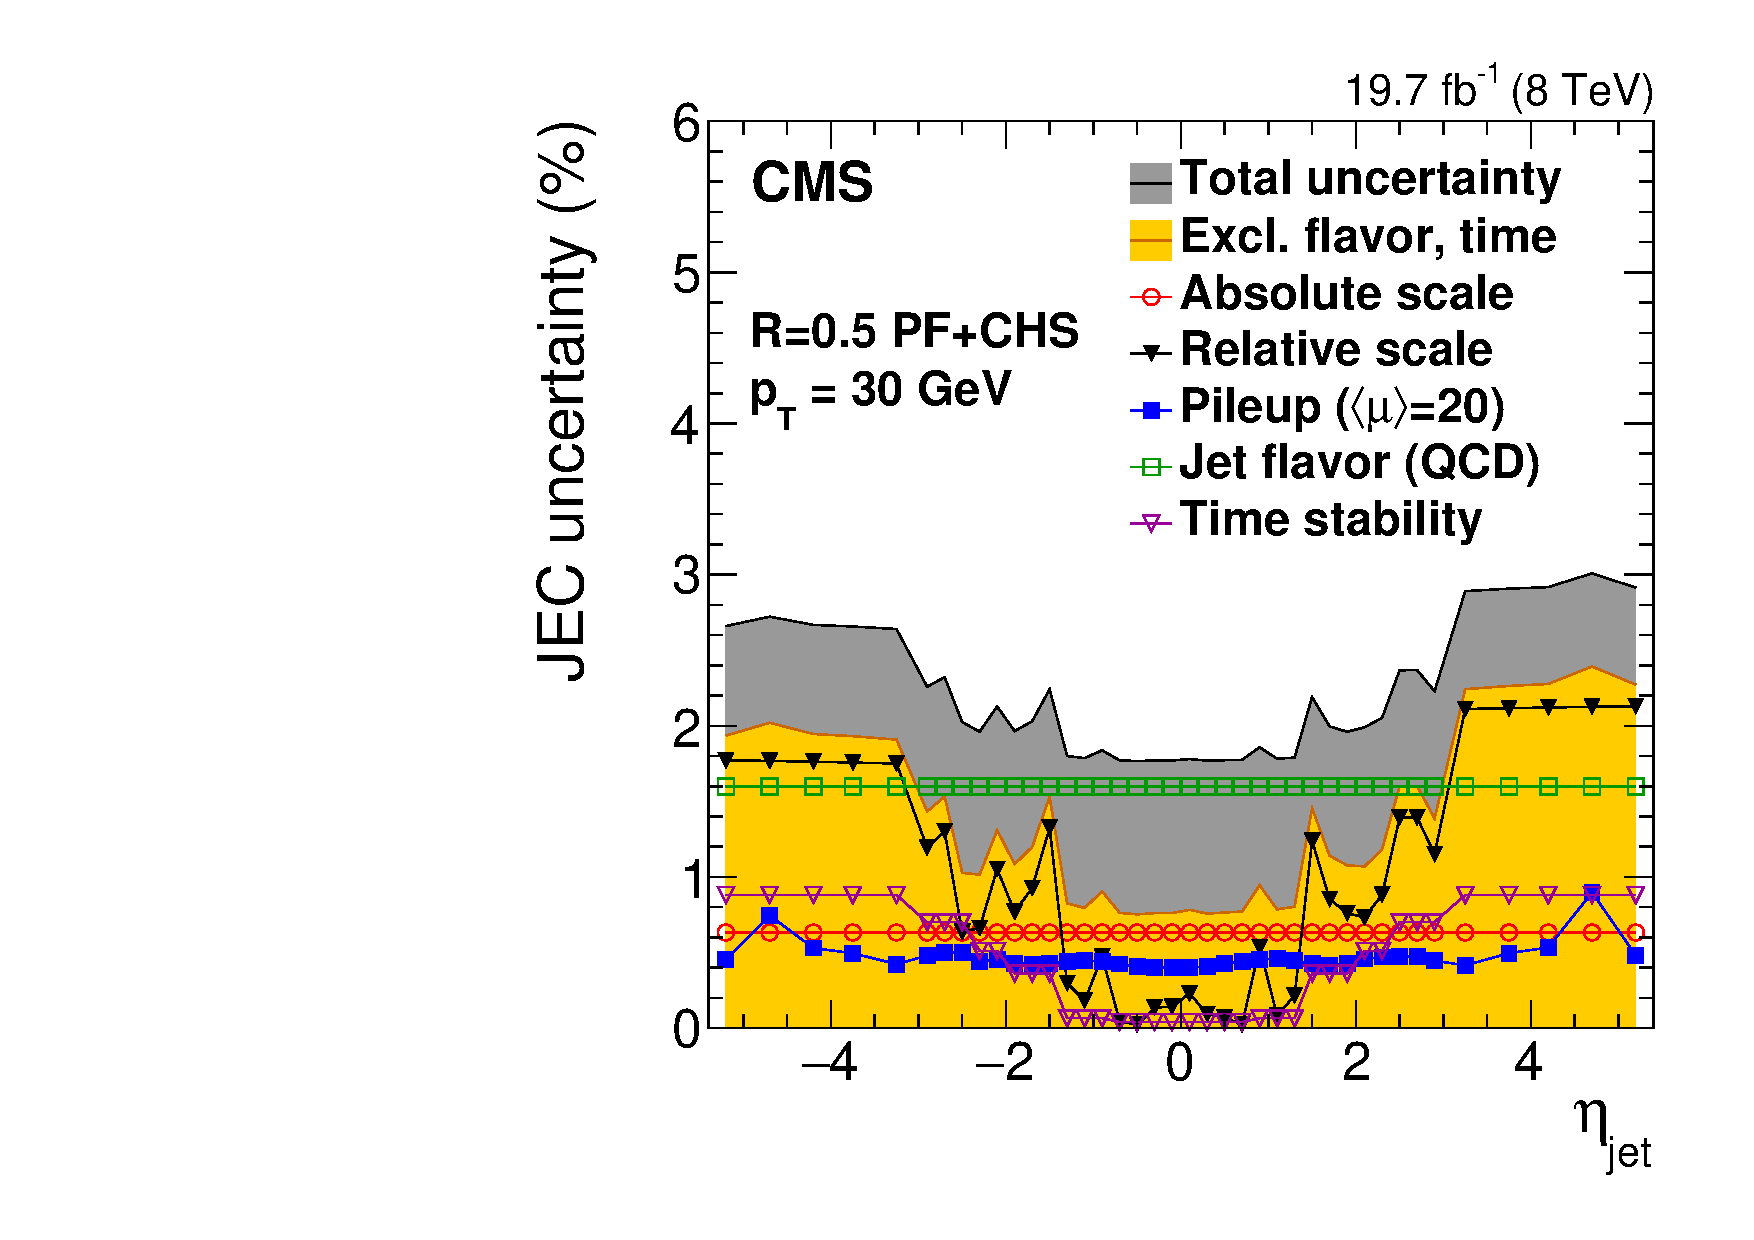
\includegraphics[width=0.49\columnwidth]{figures_chapter4/jec_unc2}
\caption{Summary of jet energy scale systematics as a function of jet $p_{T}$ for $|\eta|=0$ (left) and of jet $\eta$ for $p_{T}=30~\GeV$ at $\sqrt{s}=8~\TeV$ data taking period. The markers show the single effect of different sources and the gray dark band shows the cumulative total uncertainty. The total uncertainty, when excluding the effects of time dependence and flavor, is also shown in yellow light~\cite{Khachatryan:2016kdb}.}
\label{fig:jet_unc}
\end{figure}

Figure~\ref{fig:jet_unc} shows the summary of jet energy scale uncertainties as a function of jet $p_{T}$ and $\eta$ at $\sqrt{s}=8~\TeV$ data taking period. Jets selected for majority of the physics results are required to have a transverse momentum greater than $30~\GeV$ (the $p_{T}$ requirement is lower for jets originating from b quarks) with $|\eta|<4.7$.  The uncertainties on the jet energy scale are below $3\%$ across the phase space considered by most analyses and below $1\%$ in the barrel region when excluding the uncertainties due to jet flavor differences in the events used to derive the different stages of the jet energy scale corrections.

\subsection{Pileup Jet Identification}

Particles originating from pileup interactions can cluster into jets. The $p_{T}$ density due to pileup particles is roughly $0.7~\GeV$ per unit area in $\eta-\phi$ plane for one reconstructed primary vertex. While the pileup jets have low $p_{T}$ it is possible for these low $p_{T}$ jets to overlap and a form a single jet with relatively large $p_{T}$. The number of overlapping jets grows roughly quadratically with the number of pileup interactions and jet area~\cite{CMS-PAS-JME-13-005}.  
The goal of the pileup jet identification algorithm is to mitigate the background events due to the pileup jets. The charged particles in pileup jets generally do not point to the primary vertex of the event. In addition jets originating from pileup tend to be more diffuse in shape compared to the jets from the hard scattering. These two characteristic signatures of the pileup jets are exploited. A Boosted Decision Tree (BDT) discriminant implemented in TMVA~\cite{H�cker:1019880} is used. It takes as an input the compatibility of the tracks inside the jet with the primary vertex of the event, variables exploiting the jet shape, and the number of charged and neutral constituents of the jet. The most discriminating track related variable ($\beta^{*}$) and jet shape variable ($<\Delta R^2>$) are defined as:
\begin{eqnarray} \label{eq:pujetid}
\beta^{*} = \frac{\sum_{i \notin \mathrm{PV}} p_{Ti}}{\sum_{i} p_{Ti}}, \\
<\Delta R^{2}> = \frac{\sum_{i \in \mathrm{jet}} \Delta R^{2} p_{Ti}^2 }{\sum_{i \in jet} p_{Ti}^2},
\end{eqnarray}
where the charged particle is defined to be coming from the primary vertex if $\Delta z<0.2$ cm in the $\beta^{*}$ definition and $\Delta R$ is the distance of the particle to the jet axis in the $<\Delta R^{2}>$ definition. The distributions of these variables for "real" and pileup jets are shown in Figure~\ref{fig:pu_jet}. The $<\Delta R^{2}>$ distributions are shown for jets with $|\eta|>3.0$ where there is a degradation of separation due to the coarse granularity of the HF calorimeter. 

\begin{figure}[h]
\centering
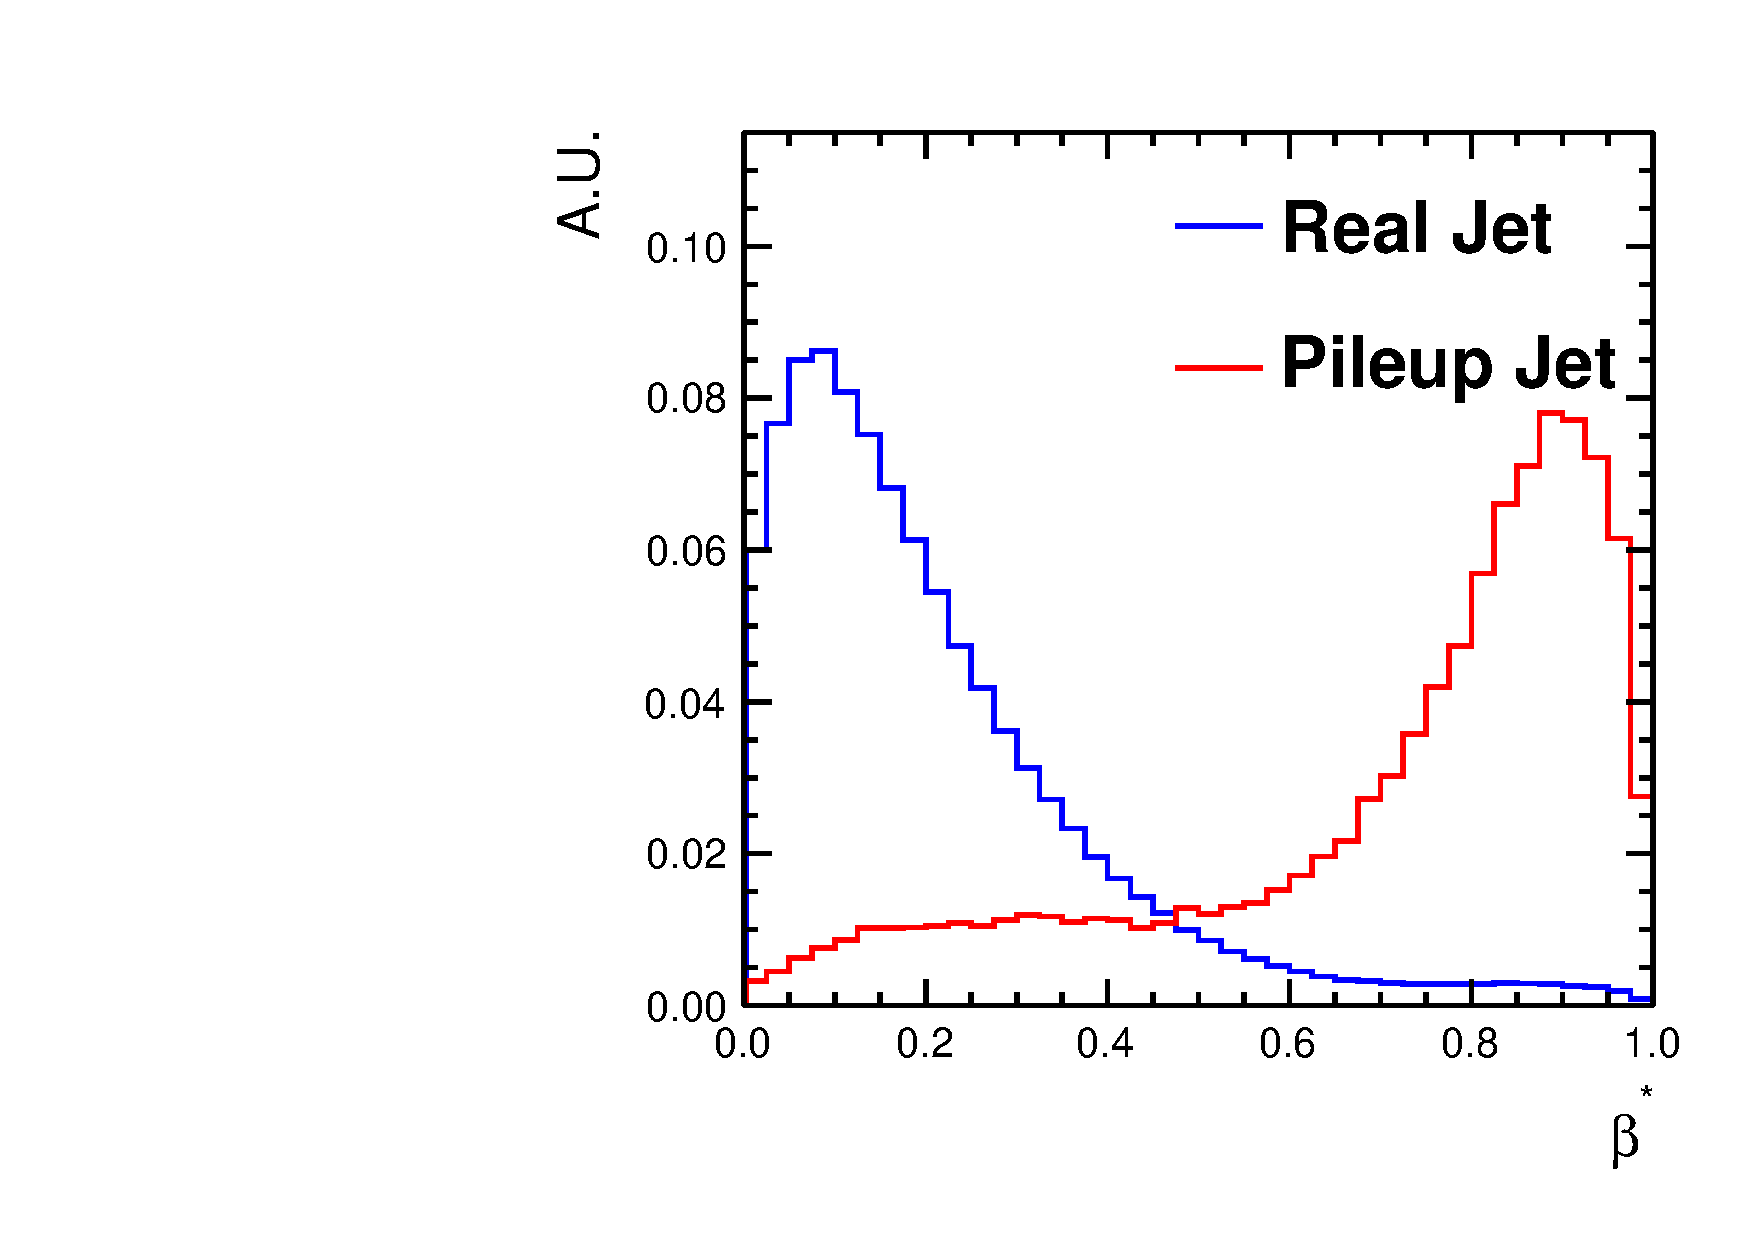
\includegraphics[width=0.49\columnwidth]{figures_chapter4/bstar}
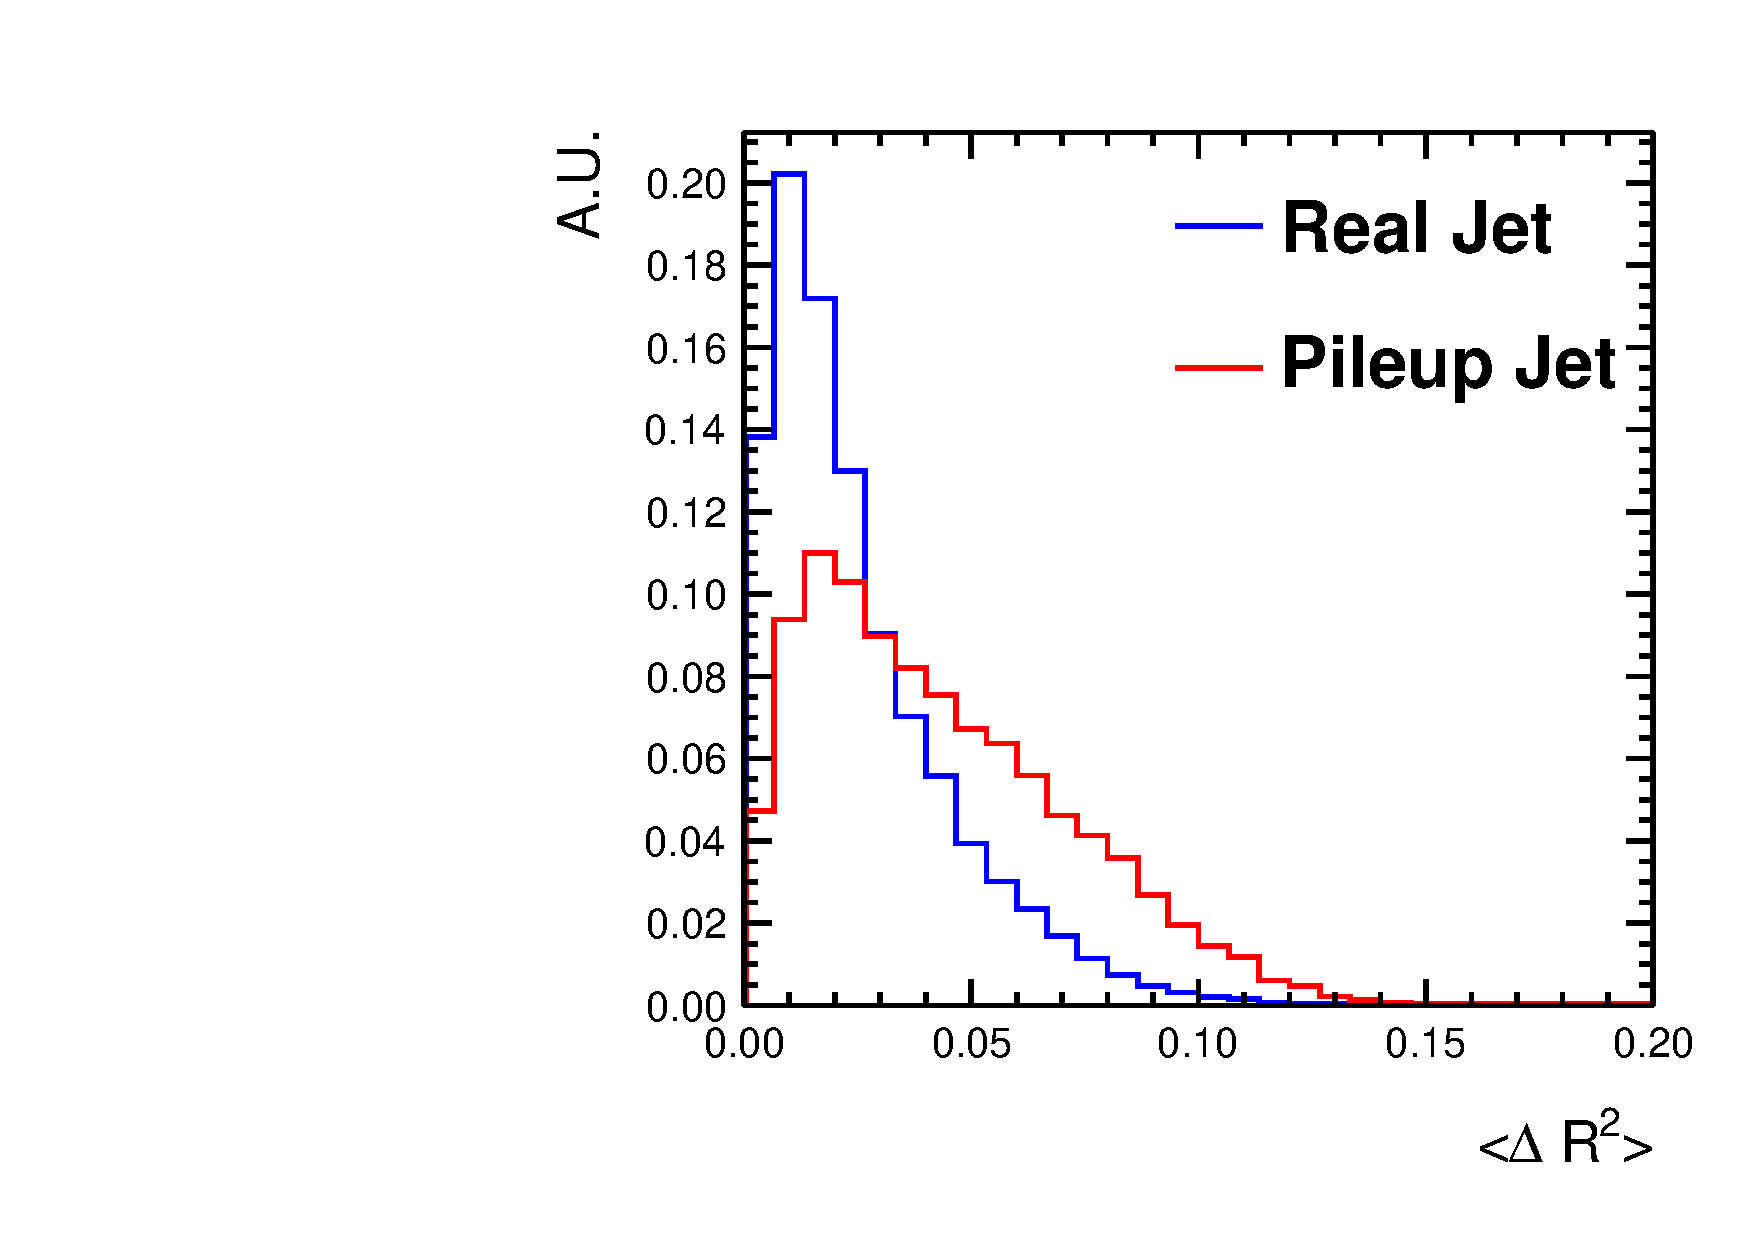
\includegraphics[width=0.49\columnwidth]{figures_chapter4/dr2}
\caption{Distributions of the $\beta^{*}$ (left panel) and $<\Delta R^{2}>$ (right panel) variables in simulation for jets matched to MC truth jet within a radius of $\Delta R<0.25$ (blue) and for jets with no match (red). Jets are required to have a $p_{T}$ greater than $25~\GeV$ and $|\eta|<2.5$ (left), and $|\eta|>3.0$ (right).}
\label{fig:pu_jet}
\end{figure}

The BDT discriminator is almost fully efficient for jets with $p_{T}>30\GeV$ in the inner tracker geometric acceptance ($|\eta|<2.4$) region with a pileup jet rejection rate of approximately $87\%$. The efficiency degrades outside of the inner tracker volume. It is about $90\%$ for "real" jets with a pileup jet rejection rate of about $40\%$ for jets with $3.0<|\eta|<5.0$.

\subsection{b-jet Identification}

The identification of jets originating from bottom quark hadronization (b-jet) is crucial to reduce the overwhelming background from processes involving jets originating from gluons, light flavored quarks, and charm quarks (c-jets).  b-jets are important signatures to study the top quark decays, the Higgs boson, and in searches for new physics. The main idea is to exploit the long lifetimes of the bottom and charm quarks and their relatively large mass. As a result one can look for secondary vertices and/or tracks with large impact parameters.  For example, the CMS inner tracking system allows to achieve an impact parameter resolution of about $15$ ($30$) $\mu$m for a track with $p_{T}$ of $100$ ($5$)~$\GeV$ while typical impact parameter values for tracks from the b-jets are at a level of a few $100$ $\mu$m~\cite{Chatrchyan:2012jua}. The so called Combined Secondary Vertex (CSV) algorithm~\cite{Chatrchyan:2012jua} is used to identify the b-jets. A likelihood discriminant is formed combining information about track impact parameters and secondary vertices. This means that the b-jets can only be identified within the inner tracker geometrical acceptance ($|\eta|<2.4$). A b-jet identification efficiency of about $75\%$ is achieved with a light-flavor jet miss-identification rate of about $1\%$. 

\section{Particle Flow}

CMS uses the so called particle flow (PF) approach to calorimetry~\cite{CMS-PAS-PFT-09-001,CMS-PAS-PFT-10-001,CMS-PAS-PFT-10-002}.  The basic idea of the PF approach is to combine information from all sub-detectors in order to reconstruct all the particles in the event using the best measurements possible. This is especially useful for jet energy measurements as roughly $62\%$ of the jet energy is carried by charged particles (mainly hadrons), around $27\%$ by photons, about $10\%$ by long lived neutral hadrons, and around $1.5\%$ by neutrinos~\cite{Thomson200925}. Thus, one can exploit the superior momentum (energy) resolution of the inner tracker (ECAL) to obtain the most accurate measurements for the charged hadrons (photons) inside the jet and within the inner tracker (ECAL) geometric acceptance. In addition, the high granularity ECAL makes it possible to separate photons from charged particle energy deposits. 

 The basic elements of the PF algorithm are tracks in the inner tracker, muon segments in the muon system, and energy clusters from the calorimeters. The calorimeter clustering allows to separate the neutral particles from the energy deposits of charged hadrons as well as to reconstruct and identify the electrons and the corresponding Bremsstrahlung photons. The clustering starts from the cluster seed defined as a local energy maxima. The clusters are then grown from the seeds by including neighboring cells, with an energy in excess of a defined threshold, in the cluster. The threshold is defined to be two standard deviation of the electronic noise of the ECAL ($80~\MeV$ in the barrel and  approximately $300~\MeV$ in the endcap) and $800~\MeV$ in the HCAL. A linking algorithm is required as a given particle will result in several PF elements. This is achieved by defining a distance measure between each pair of PF elements. For example, the ECAL clusters of bremsstrahlung photons emitted by an electron are linked by extrapolating the tangents of the track at each intersection point with an inner tracking detector layer to the ECAL to form a PF block. It has to be noted that due to high granularity of the CMS detector the linked blocks typically contain only $1-3$ elements. The PF candidates are identified from these blocks. 
 
 The block and the corresponding PF elements are iteratively removed from further consideration once a PF candidate has been identified. A global muon is denoted as a PF muon if a track element is compatible with the global muon. The track is removed from further consideration and the expected energy deposits in the calorimeters are subtracted from the corresponding calorimeter clusters.  The GSF electron tracks are linked to the ECAL clusters using a discriminator against charged pions that utilizes information from the inner tracker and the ECAL. A PF electron is formed from the GSF tracks and the ECAL clusters (including the clusters identified as bremsstrahlung photons) in case of a positive match. The remaining inner tracker tracks are identified as charged hadrons. If the linked calorimeter cluster energy exceeds the tracker momentum (taking the relevant measurement uncertainties into account) the energy excess is identified as a neutral particle. In addition a PF photon is identified if the excess energy is larger than the linked ECAL cluster while the remaining energy is assigned to a neutral hadron. The remaining ECAL (HCAL) clusters that do not have a linked track are denoted as PF photons (PF neutral hadrons).   
 
 The output of the PF algorithm are denoted as particle flow candidates and are classified as electrons, photons, muons, charged hadrons, or neutral hadrons. The particle flow candidates are used for the reconstruction of jets (referred as PF jets) as described in the previous section. A special version of the PF algorithm is used in the HLT optimized to the HLT requirements. 

\section{Hadronic Tau Decays}

The $\tau$ lepton with a mass of $1.777~\GeV$~\cite{Agashe:2014kda} is the only lepton sufficiently heavy to be able to decay to hadrons.  Hadronic tau decays proceed via weak interaction into one or three charged pions or kaons with up to two neutral pions, and one tau neutrino ($\nu_{\tau}$). The $\nu_{\tau}$ escapes the detector resulting in a missing energy in the event. The $\pi_{0}$ meson decays almost exclusively to a pair of photons. Table~\ref{tab:tau_decay} summarizes the most common hadronic tau decays. The mean lifetime of the $\tau$ lepton is $290\times10^{-15}$ s~\cite{Agashe:2014kda} resulting in a significant (compared to the transverse impact parameter and secondary vertex resolution) displacement of the decay vertex from the production vertex for energetic taus. The hadronic tau decays are denoted as $\tau_{h}$ henceforth. The tau decays to muons and electrons are denoted as $\tau_{\mu}$ and $\tau_{e}$ respectively.  

\begin{table}[htbp]
\begin{center}
\begin{tabular}{lcc} 
\hline 
Decay Mode & Resonance  & Branching fraction $[\%]$   \\ 
\hline 
$\tau^{\pm} -> h^{\pm} \nu_{\tau}$                             &             & 11.5 \\
$\tau^{\pm} -> h^{\pm} \pi^{0} \nu_{\tau}$                    & $\rho(770)$ & 26.0 \\
$\tau^{\pm} -> h^{\pm} \pi^{0}  \pi^{0} \nu_{\tau}$            & $a_1(1260)$            & 10.8 \\
$\tau^{\pm} -> h^{\pm} h^{\pm} h^{\mp} \nu_{\tau} $            & $a_1(1260)$            & 9.8 \\
$\tau^{\pm} -> h^{\pm} h^{\pm} h^{\mp} \pi^{0} \nu_{\tau} $ &                         & 4.8 \\
Other hadronic modes &                         & 1.8 \\ 
\hline 
All hadronic modes &                         & 64.8 \\ 
\hline 
\end{tabular}
\caption{Approximate branching fractions of hadronic tau decay modes~\cite{Agashe:2014kda}. The intermediate meson resonances are indicated where appropriate. The symbol $h$ represents a charged pion or kaon.
}
\label{tab:tau_decay}
\end{center}
\end{table}

The visible decay products in the $\tau_{h}$ decays result in collimated jets with a relatively low particle multiplicity. The main idea of the $\tau_{h}$ reconstruction algorithm is to reconstruct the individual decay modes listed in Table~\ref{tab:tau_decay}. The hadron-plus-strip (HPS) algorithm~\cite{1748-0221-7-01-P01001} takes advantage of the PF algorithm using the reconstructed charged and neutral PF candidates.  The HPS algorithm starts with a PF jet of $p_{T}$ greater than $14~\GeV$ and $|\eta|<2.5$ using the anti-$k_{T}$ algorithm with distance parameter of $R=0.5$. The photons produced in $\pi^{0} \rightarrow \gamma\gamma$ decays are likely to convert to an electron-positron pair within the volume of the inner tracker. This is taken into account by clustering the electrons and photons (with $p_{T}>0.5~\GeV$)  in the jet into strips in the $\eta-\phi$ plane with a window size of $0.05\times0.20$ taking the direction of the bending of the charged trajectories into account. Strips with total $p_{T}$ sum larger than $2.5~\GeV$ are identified as $\pi^{0}$ candidates. 

$\tau_{h}$ candidates are formed by combining the clustered strips with the charged candidate constituents of the jets. The charged particles are required to have a $p_{T}$ greater than $0.5~\GeV$. The distance of closest approach to the charged particle of highest $p_{T}$ in the jet has to be less than $0.4$ cm in the $z$ direction and $0.03$ cm in the transverse plane~\cite{1748-0221-11-01-P01019}. The following decay hypotheses are considered:

\begin{description}
\item[$\bullet$ $h^{\pm}$:] A single charged particle with no $\pi^{0}$ candidates.  
\item[$\bullet$ $h^{\pm} \pi^{0}$:] One charged particle and one strip with a system mass of $0.3<m_{\tau_{h}}<1.3~\GeV$ for $p_{T}<200~\GeV$. The size of the mass window is enlarged for $\tau_{h}$ candidates with high $p_{T}$ to account for the inner tracker momentum resolution degradation. The mass cut utilizes the intermediate meson resonance ($\rho(770)$) mass in the decay. 
\item[$\bullet$ $h^{\pm} \pi^{0}  \pi^{0}$:] One charged particle combined with two strips. The mass cut requirement is $0.4<m_{\tau_{h}}<1.2~\GeV$ for $p_{T}<200~\GeV$ targeting the intermediate meson resonance decay of $a_{1} (1260)$.  The size of the mass window is enlarged for $\tau_{h}$ candidates with high $p_{T}$.
\item[$\bullet$ $h^{\pm} h^{\pm} h^{\mp}$:] A combination of three charged particles with a system mass of $0.8<m_{\tau_{h}
}<1.5~\GeV$. The sum of the charges is required to be $1$. The charged tracks are required to originate from the same event vertex ($\Delta z< 4$ mm).
\end{description}

\begin{figure}[h]
\centering
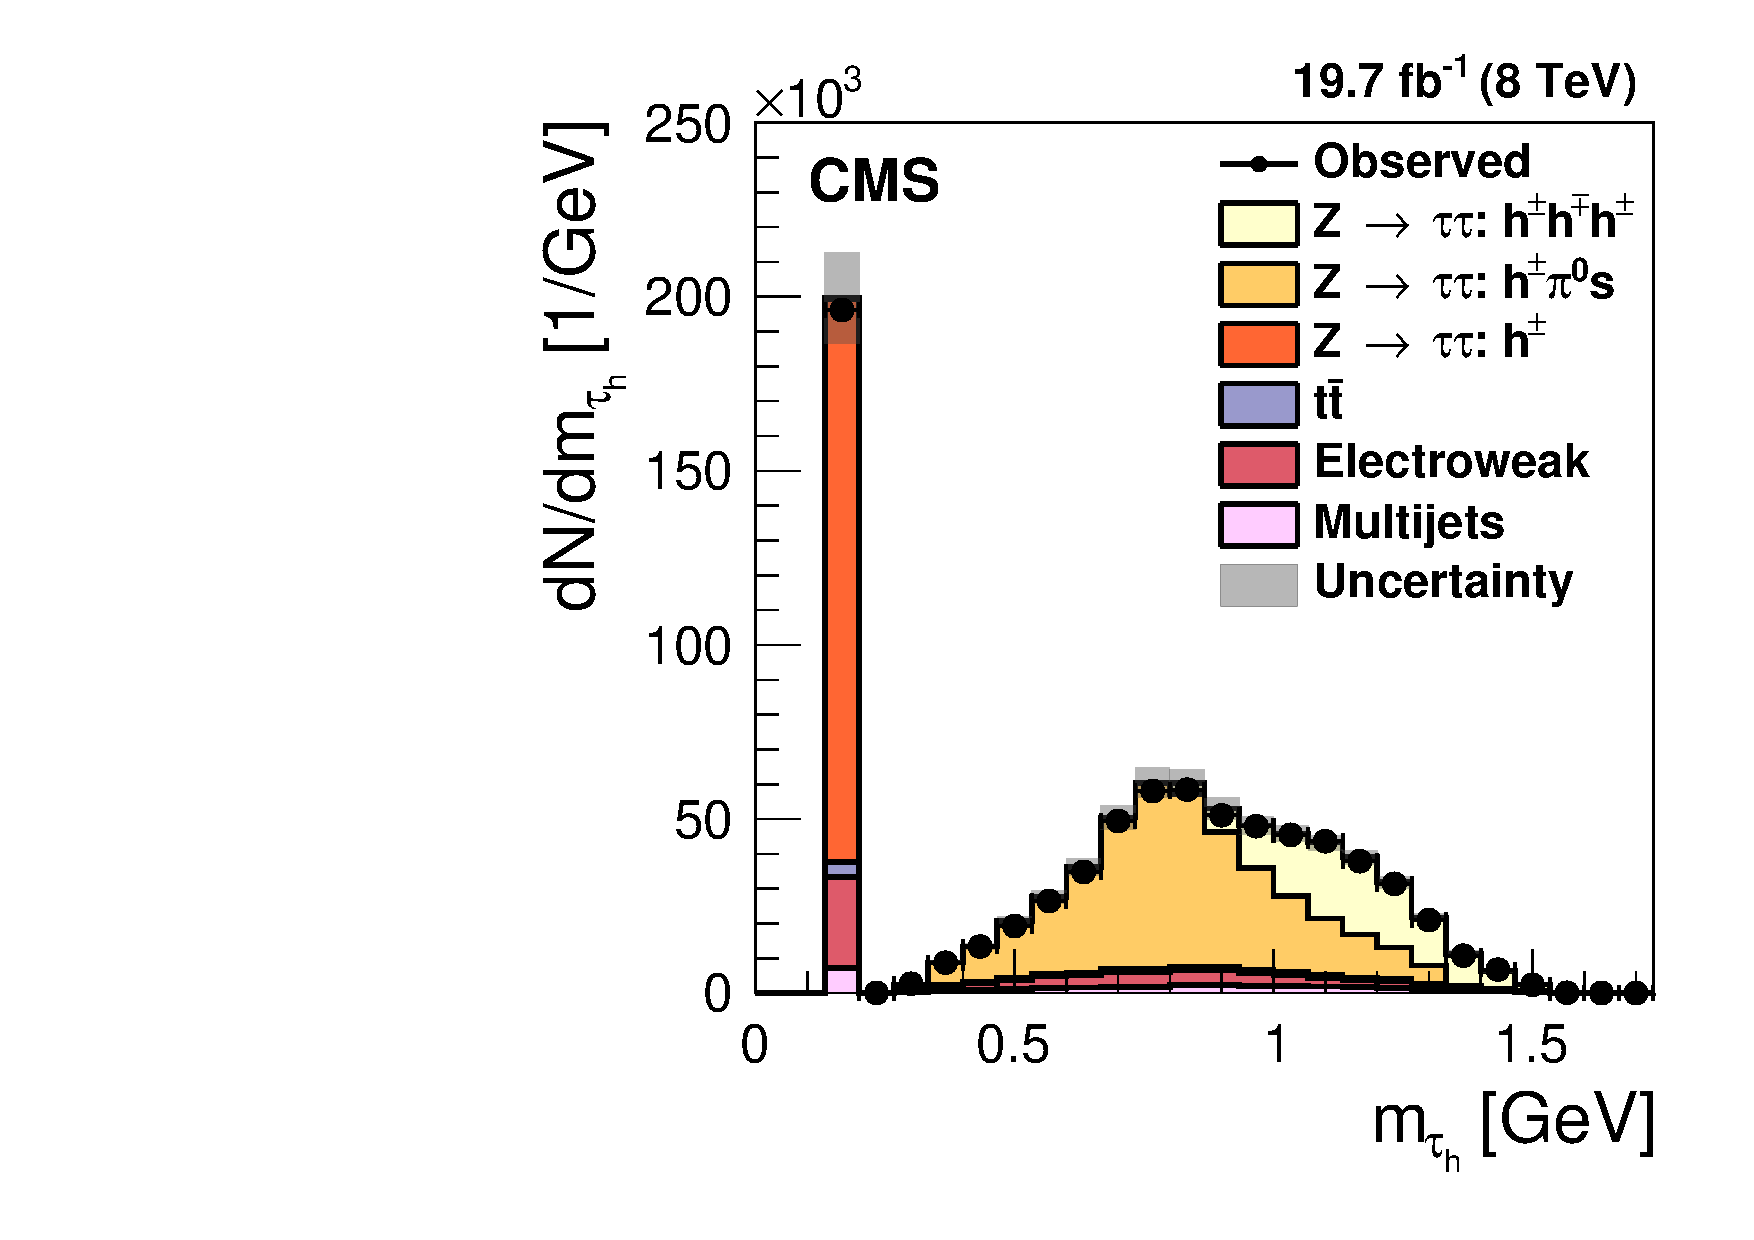
\includegraphics[width=0.80\columnwidth]{figures_chapter4/tau_mass}
\caption{Distribution of the $\tau_{h}$ masses in $Z/\gamma^{*} \rightarrow \tau\tau$ events selected in data during $\sqrt{s}=8~\TeV$ data taking period. Expected predictions from the simulation are also shown. The $Z \rightarrow \tau\tau$ prediction is split into the different expected $\tau_{h}$ decay modes. The electroweak background is mainly due to $W+$jets production~\cite{1748-0221-11-01-P01019}.}
\label{fig:tau_mass}
\end{figure}

An additional requirement is imposed on the separation of the charged hadrons and strips. All the charged hadrons and strips are required to be within a narrow cone of $\Delta_R = 3.0 /p _{T}~[\GeV]$ around the jet axis to exploit the collimation of the decay products of energetic taus. When $\Delta_R$ is smaller than $0.05$ or exceeds $0.10$, a cone size of $0.05$ or $0.10$ is used respectively. Figure~\ref{fig:tau_mass} shows the distribution of the mass of $\tau_{h}$ for $Z/\gamma^{*} \rightarrow \tau\tau$ events at $\sqrt{s}=8~\TeV$ data taking period. The individual decay modes are highlighted by splitting the simulated $Z/\gamma^{*} \rightarrow \tau\tau$ events according to the reconstructed $\tau_{h}$ decay mode. As one can see the $m_{\tau_h}$ distribution peaks around the intermediate meson resonance masses of $\rho(770)$ and $a_{1}(1260)$. The narrow peak near the charged pion mass is due to the single charged particle decay mode. 

Jets originating from quarks and gluons remain a large background to the $\tau_{h}$ reconstruction. This background is further reduced by requiring the selected $\tau_{h}$ candidates to be isolated. The $\tau_{h}$ candidate isolation is discussed in the next section. It is also possible for an electron or muon to be miss-identified as a $\tau_{h}$ candidate. For example, an electron with a radiated bremsstrahlung photon that undergoes a pair conversion is likely to be reconstructed as a $h^{\pm} \pi^{0}$ decay mode.  Miss-identified muons are rejected if track segments are found in at least two muon stations consistent with the direction of the $\tau_{h}$ candidate. There are also additional requirements on the expected energy deposits in the ECAL and HCAL. Miss-identified electrons are rejected by considering variables sensitive to the distribution of the energy deposits in the ECAL and the particle multiplicities to distinguish electromagnetic and hadron showers. Variables sensitive to the  bremsstrahlung radiation are also considered. For example, the amount of bremsstrahlung radiation can be quantified by $\frac{p_{in}-p_{out}}{p_{in}}$  where $p_{in}$ ($p_{out}$) is the measured momentum at the innermost (outermost) region of the inner tracker. A BDT discriminant is implemented taking as an input these variables. More details can be found in~\cite{1748-0221-11-01-P01019}. 

\section{Lepton Isolation}

Leptons originating from the decays of the $W$, $Z$, and Higgs bosons are expected to be isolated from additional hadronic activity in the vicinity of  the lepton. On the other hand, the leptons originating from the decays of the bottom and charm quarks and in-flight decays of the kaons and pions are surrounded by a significant contribution of additional hadrons present inside the jet. It is also possible for a charged hadron inside a jet to be miss-reconstructed as a lepton. Thus, in either of these cases the lepton candidates have a significant energy flow in the vicinity of the lepton trajectory and a requirement on the isolation reduces these lepton backgrounds.

The PF candidates are used to define the isolation metric as this ensures that the most accurate measurements are used. Moreover, the use of the PF candidates avoids a possible double counting where the energy deposits of the same particle in different sub-detectors are included in the isolation metric. The isolation metric for the muons and electrons is defined as:
\begin{eqnarray} \label{eq:isolation2}
I_{\ell} = \sum_{i \in \mathrm{PV}} p_{iT}^{\mathrm{charged}} + \sum_{i} (p_{iT}^{\mathrm{neutral}}+p_{iT}^{\gamma})-p_{T}^{\mathrm{PU}},
\end{eqnarray}
where the charged and neutral particles are required to be within a cone of radius $\Delta R=0.4$ around the lepton direction. The lepton, the neutral hadrons, and photons in the innermost region of the cone ($\Delta R<0.01$) are excluded from the isolation sum to take into account the radiation off the lepton. The isolation metric defined in Eq.~(\ref{eq:isolation2}) is susceptible to the additional pileup interactions present in the event. The contribution of the charged particles originating from the pileup interactions are removed by considering only the charged particles associated to the primary vertex of the event. This is achieved by only including the charged particles within $0.1$ cm of the closest approach of the corresponding track to the primary vertex in the $z$ coordinate.

The last term in Eq.~(\ref{eq:isolation2}) denotes the contribution of the neutral particles originating from the pileup interactions. Two methods are used to estimate the $p_{T}^{\mathrm{PU}}$. The first method is based on the observation that the rate of the charged particles originating from the pileup interactions is about two times larger than the corresponding rate of the neutral particles. Thus, the contribution due to the neutral particles originating from the pileup interactions can be estimated by determining the contribution of the charged particles not associated to the primary vertex: 
\begin{eqnarray} \label{eq:pu}
p_{T}^{\mathrm{PU}} = \frac{1}{2} \sum_{i \notin \mathrm{PV}} p_{iT}^{\mathrm{charged}}.
\end{eqnarray}
Only the charged particle contribution is included in the isolation sum if the magnitude of the $p_{T}^{\mathrm{PU}}$ is larger than the neutral contributions in Eq.~(\ref{eq:isolation2}). The second method is based on calculating the median energy density $\rho$ of the pileup interactions in the isolation cone similar to the jet area method discussed in section 3.5.1. This method is used for the electron isolation metric~\cite{Khachatryan:2015hwa}. Selected electrons and muons are required to be isolated by applying a requirement on the relative isolation $\frac{I_{\ell}}{p_{T}^{\ell}}$ where $p_{T}$ is the lepton transverse momentum. A relative isolation values less than $0.10$ to $0.15$ are typically required for the selected lepton candidates depending on the $\eta$ region. The exact values are optimized for each data taking period.  

\begin{figure}[h]
\centering
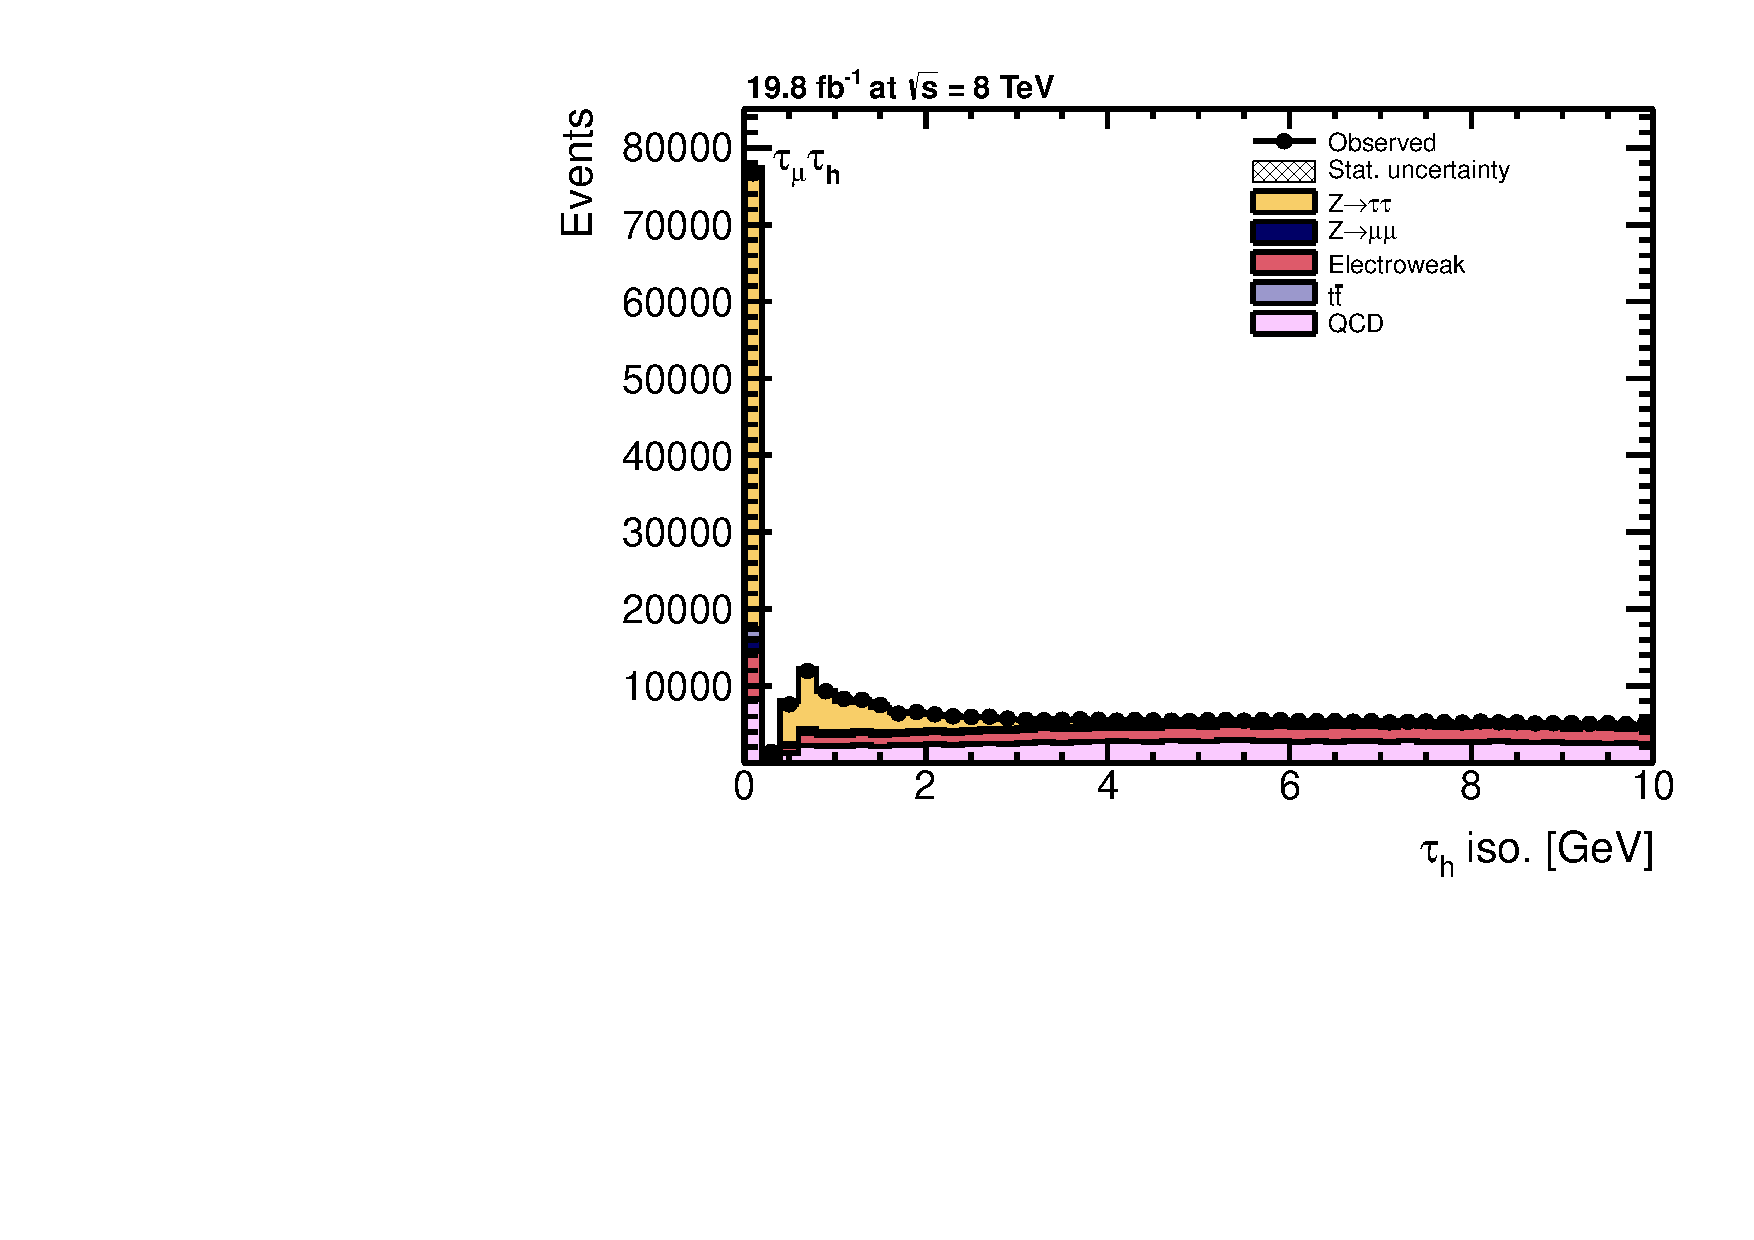
\includegraphics[width=0.80\columnwidth]{figures_chapter4/tauiso}
\caption{Distribution of $\tau_{h}$ isolation for $\tau^{+}\tau^{-}$ candidates events with a muon and $\tau_{h}$ final state with $p_{T}>20~\GeV$. Points represent the data and the histograms show the expected contribution from different SM processes. The muon selection requirement on the isolation is $I_{\mathrm{rel}}<0.1$. The QCD multi-jet process contributions is estimated from same-sign charged muon and $\tau_{h}$ and the electroweak background is mainly due to $W+$jets production. The $W+$jet contribution is suppressed here by a selection requirement on the transverse mass of the muon and missing transverse energy system as discussed in the next chapter.}
\label{fig:tau_iso}
\end{figure}

The charged hadrons used to reconstruct the tau hadronic decays and the electrons and photons used to form the strips are excluded from the isolation sum for the $\tau_{h}$ isolation. The Eq.~(\ref{eq:isolation}) is slightly modified for the $\tau_{h}$ isolation definition:
\begin{eqnarray} \label{eq:isolation}
I_{\tau_{h}} = \sum_{i \in \mathrm{PV}} p_{iT}^{\mathrm{charged}} + \mathrm{max} (0,\sum_{i} p_{iT}^{\gamma}-0.46 \sum_{i \notin \mathrm{PV}} p_{iT}^{\mathrm{charged}}),
\end{eqnarray}
where a cone size of $\Delta R=0.5$ around the $\tau_h$ direction is used and the $p_{T}$ of the charged hadrons and photons is required to be greater than $0.5~\GeV$. The track distance requirement to the primary vertex is $0.2$ cm in the $z$ direction and $\Delta r<0.03$ cm in the transverse direction. A cone size of $\Delta R=0.8$ around the $\tau_h$ direction is used to compute the contribution of the charged particles originating from the pileup interactions. The factor $0.46$ minimizes the dependance of the efficiency of the isolation to the pileup interactions. Figure~\ref{fig:tau_iso} shows the distribution of the $I_{\tau_h}$ for $\tau^{+}\tau^{-}$ candidate events with a muon and $\tau_{h}$ final state with $p_{T}>20~\GeV$. Events with large $I_{\tau_h}$ values mainly come from QCD multi-jet background and $W+$jet events where the $W$ decays to a muon and a jet is miss-identified as a $\tau_{h}$. The $W+$jet contribution is suppressed here by a selection requirement on the transverse mass of the muon and missing transverse energy system as discussed in the next chapter. The selected $\tau_{h}$ candidates are required to have $I_{\tau_h}$ values less than $1.0~\GeV$ for the $\tau_{h}\tau_{h}$ final states and $1.5~\GeV$ for the $\tau_{\ell}\tau_{h}$ final states. The efficiency to select the $\tau_{h}$ candidates ranges from $60\%$ to $70\%$ with a jet miss-identification probability of about $1\%$~\cite{1748-0221-11-01-P01019}.  Figure~\ref{fig:tau_iso} shows that relaxing the requirements on the lepton isolation provides a useful control region enriched with the background processes with a jet is miss-identified as a lepton.   

\section{Missing Transverse Energy}

Neutrinos and hypothetical neutral weakly interacting particles produce a momentum imbalance in the plane perpendicular to the beam direction. The missing transverse momentum $\vec{E}_{T}^{miss}$ is defined as the negative vectorial sum of all the visible particle transverse momenta in the event. The magnitude $E_{T}^{miss}$ is referred to as the missing transverse energy. A precise measurement of $E_{T}^{miss}$ is crucial for the $W$ boson cross section measurements and plays a key role in the Higgs boson searches decaying to $\tau\tau$ final states. Precise calibration of all the reconstructed physics objects in the event is important for the $\vec{E}_{T}^{miss}$ performance. Therefore, the PF candidates are used to reconstruct the $\vec{E}_{T}^{miss}$:
\begin{eqnarray} \label{eq:met}
\vec{E}_{T}^{miss} = - \sum_{i \in{\mathrm{PF candidates}}} \vec{p}_{Ti},
\end{eqnarray}
denoted as PF $\vec{E}_{T}^{miss}$. 

The  $\vec{E}_{T}^{miss}$ response and resolution can be degraded due to minimum energy thresholds and non-linear response in the calorimeters, and $p_{T}$ thresholds and inefficiencies in the inner tracker. By correcting the jet energy scale as described above one can reduce the biases in the response of $\vec{E}_{T}^{miss}$ introduced by these effects\cite{Khachatryan:2014gga}. In addition, the $\vec{E}_{T}^{miss}$ is sensitive to the additional pileup interactions in the event. While contribution of genuine $\vec{E}_{T}^{miss}$ from the pileup interactions is small due to small probability to produce neutrinos in the inelastic $pp$ collisions, the nonlinearity and minimum thresholds of the calorimeters cause the $\vec{E}_{T}^{miss}$ to point on average in the direction of the vectorial $\vec{p}_{T}$ sum of the neutral particles. Each additional pileup interaction in a given event degrades the resolution of the PF $\vec{E}_{T}^{miss}$ by about $3.5~\GeV$ added in quadrature~\cite{Khachatryan:2014gga}. On the other hand the impact on the response of the PF $\vec{E}_{T}^{miss}$ is small as the additional pileup interactions are isotropic.  

\begin{figure}[h]
\centering
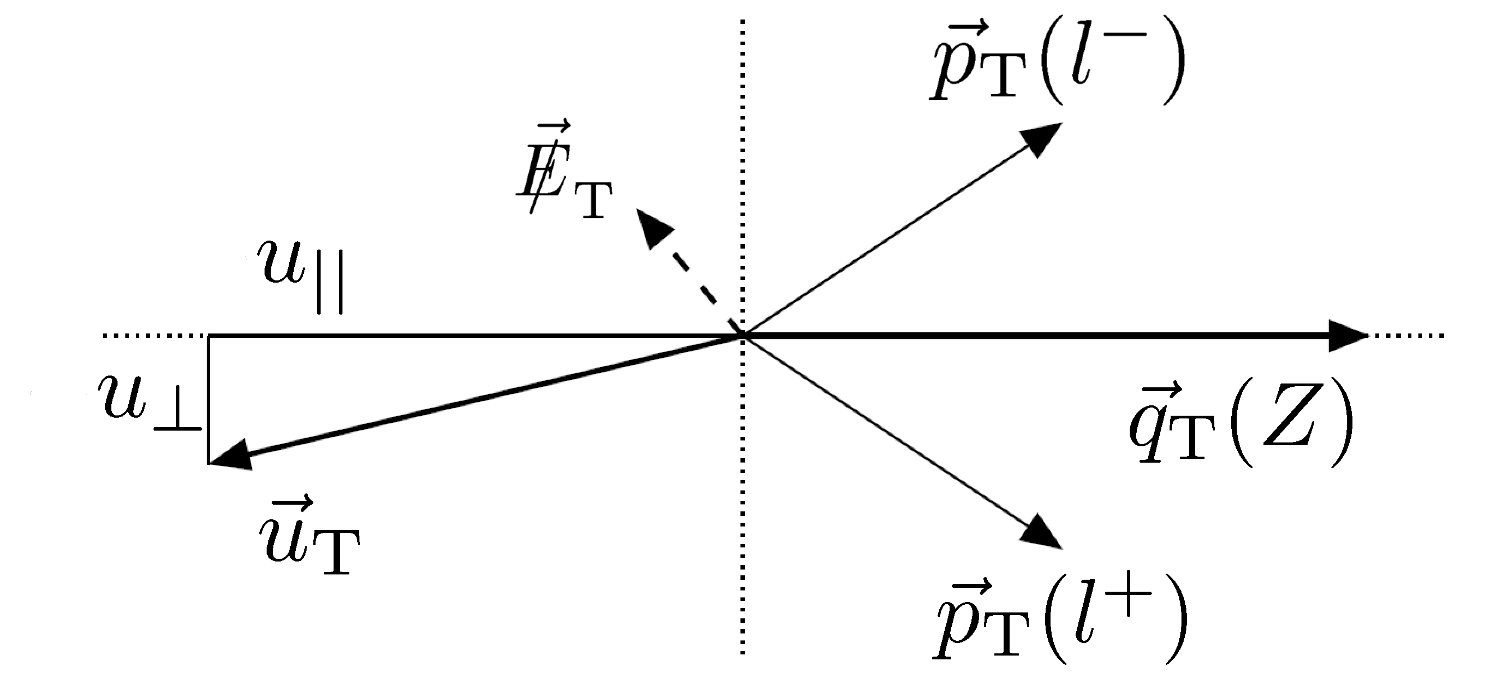
\includegraphics[width=0.49\columnwidth]{figures_chapter4/recoil}
\caption{Illustration of the recoil $\vec{u}_{T}$ definition in the transverse plane for $Z \rightarrow \ell \ell$ events~\cite{Khachatryan:2014gga}.}
\label{fig:recoil_def}
\end{figure}

Thus, it is crucial to mitigate the effect of the pileup interactions on the resolution of the $\vec{E}_{T}^{miss}$. Two methods are employed in the results shown in the next chapter. The main approach in both of these methods is to identify the particles that are likely to originate from the pileup interactions and the particles that are likely to originate from the hard scattering of interest. MVA PF $\vec{E}_{T}^{miss}$ method relies on a BDT regression algorithm as implemented in TMVA~\cite{H�cker:1019880}.  Consider a $W \rightarrow \ell \nu$ event. The hadronic recoil is defined as: 
\begin{eqnarray} \label{eq:met}
\vec{u}_{T} = - \vec{q}_{T} -\vec{E}_{T}^{miss},
\end{eqnarray}
where $\vec{q}_{T}$ is the transverse momentum of the $W$ boson. The recoil can be identically defined for the $Z \rightarrow \ell\ell$ events even though there is no genuine $\vec{E}_{T}^{miss}$ in this process. The $Z$ boson can be well measured in these events allowing to better understand the response and resolution of the recoil. The $\vec{q}_{T}$ of the $Z$ boson defines a unique axis in the event. The hadronic recoil is projected onto this axis to obtain the parallel $u_{\parallel}$ and perpendicular  $u_{\bot}$  components of the recoil. This is illustrated in Figure~\ref{fig:recoil_def}. The BDT regression first corrects the recoil direction to the true hadronic recoil direction. The magnitude of the $\vec{u}_{T}$ is corrected in the second step using simulated $Z \rightarrow \mu\mu$ and $\gamma+$jets events. The BDT utilizes $5$ different constructions of the recoil ($\vec{E}_{T}^{miss}$):  
\begin{figure}[h]
\centering
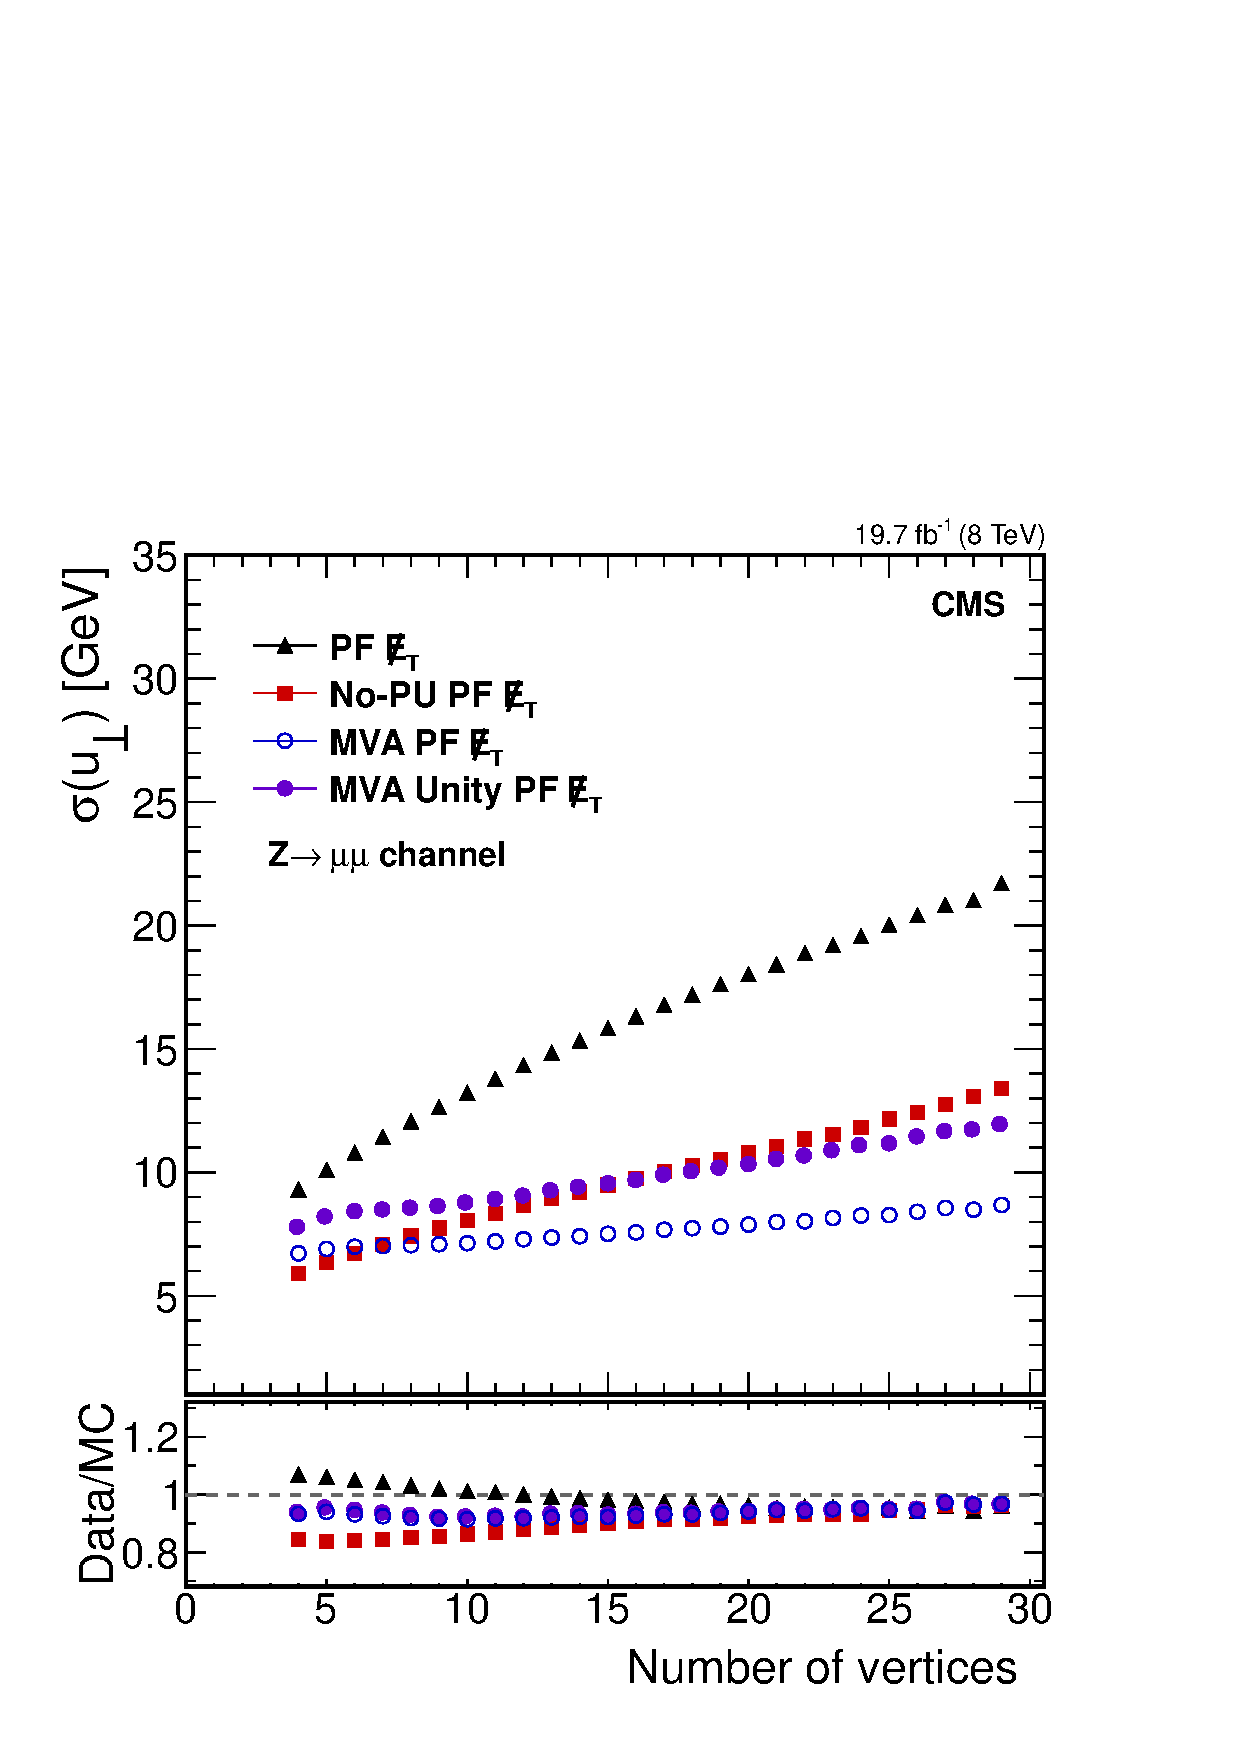
\includegraphics[width=0.49\columnwidth]{figures_chapter4/mva_met}
\caption{The resolution of the perpendicular component of the recoil as a function of the number of vertices for $Z \rightarrow \mu\mu$ data events shown for the PF $\vec{E}_{T}^{miss}$ in black triangles and MVA MVA PF $\vec{E}_{T}^{miss}$ in blue open circles for the $\sqrt{s}=8~\TeV$ data taking period. The MVA Unity PF $\vec{E}_{T}^{miss}$ and No-PU PF $\vec{E}_{T}^{miss}$ are additional pileup mitigation techniques not discussed here~\cite{Khachatryan:2014gga}.}
\label{fig:resolution}
\end{figure}
\begin{description}
\item[$\bullet$] The negative sum $\vec{p}_{T}$ of all the PF candidates. The standard definition of the  PF $\vec{E}_{T}^{miss}$. 
\item[$\bullet$] The negative sum $\vec{p}_{T}$ of all the charged PF candidates associated to the primary vertex of the event.   
\item[$\bullet$] The negative sum $\vec{p}_{T}$ of all the charged PF candidates and all the neutral PF candidates inside jets satisfying the pileup jet identification requirement discussed in section  3.5.2.
\item[$\bullet$] The negative sum $\vec{p}_{T}$ of all the charged PF candidates not associated to the primary vertex of the event and all the neutral PF candidates within jets not satisfying the pileup jet identification requirement.
\item[$\bullet$] The negative sum $\vec{p}_{T}$ of all the charged PF candidates associated to the primary vertex of the event and all the neutral PF candidates. In addition, the PF candidates within jets not satisfying the pileup jet identification requirement are added to this sum $\vec{p}_{T}$.
\end{description}
Figure~\ref{fig:resolution} shows the the resolution of the perpendicular component of the recoil as a function of the number of reconstructed vertices in $Z \rightarrow \mu\mu$ data events at $\sqrt{s}=8~\TeV$ data taking period. The black triangles show the PF $\vec{E}_{T}^{miss}$ and the blue open circles show the MVA $\vec{E}_{T}^{miss}$. As it can be seen the resolution of the PF $\vec{E}_{T}^{miss}$ is significantly degraded with additional pileup interactions in the event while the MVA PF $\vec{E}_{T}^{miss}$ resolution is significantly better compared to the PF $\vec{E}_{T}^{miss}$ resolution. For example, for the $\sqrt{s}=8~\TeV$ data taking period the average number of pileup interactions is $20$ (Figure~\ref{fig:pu}) resulting in the improvement of the MVA PF $\vec{E}_{T}^{miss}$ resolution by a factor of two with respect to the PF $\vec{E}_{T}^{miss}$ resolution. 

The second method used to mitigate the effect of the additional pileup interactions in the event is called pileup per particle identification (PUPPI)~\cite{Bertolini:2014bba}. The main idea consists of defining a shape variable that encodes the collinear versus soft diffuse structure around a given particle. The charged particles within the inner tracker acceptance region not associated to the primary vertex are used to compute the shape variable distribution for each event. An assumption is made that this distribution is representative of all the particles originating from the pileup interactions. The shape variable is then used to define a weight associated with each particle giving the probability of that particle to originate from a pileup interaction. The charged particles associated to the primary vertex are assigned a weight of $1$ while the charged particles not associated to the primary vertex are assigned a weight of $0$. The weights are then used to rescale the four-momenta of the particles. The particles with very small weights or transverse momentum are discarded. The PUPPI $\vec{E}_{T}^{miss}$ is determined by the negative $\vec{p}_T$ sum of the rescaled four-momenta of the PF candidates. The PUPPI $\vec{E}_{T}^{miss}$ resolution is comparable to the resolution obtained using the MVA $\vec{E}_{T}^{miss}$ technique.

\subsection{Recoil Calibration}

Discrepancies between simulation and data in the response and resolution of the recoil are calibrated using the $Z \rightarrow \mu\mu$ data events. Figure~\ref{fig:resolution} shows the simulation and data differences in the lower panel of the figure. The differences are due to imperfect simulation of the underlying event, and  differences in the calorimeter response and resolution. The distributions of the parallel and perpendicular components of the recoil in the $Z \rightarrow \mu\mu$ data and simulation events are fitted with a double Gaussian. This is done as a function of the $Z$ boson $p_{T}$ and the number of reconstructed jets in the event. Figure~\ref{fig:recoil} shows a typical fit for the recoil parallel (left panel) and perpendicular (right panel) components in the $Z \rightarrow \mu\mu$ data at $\sqrt{s}=13~\TeV$ data taking period.   
\begin{figure}[h]
\centering
\includegraphics[width=0.49\columnwidth]{figures_chapter4/pfu1fit_1}
\includegraphics[width=0.49\columnwidth]{figures_chapter4/pfu2fit_1}
\caption{Double Gaussian fits to the distributions of the parallel (left panel, denoted as $u_{1}$) and perpendicular (right panel, denoted as $u_{2}$) components of the recoil in $Z\rightarrow\mu\mu$ data events at $\sqrt{s}=13~\TeV$ data taking period. The fits are shown for the $Z$ $p_{T}$ in the range of $10$ to $20~\GeV$. The PUPPI algorithm is used for the recoil distributions shown here. The $\sigma_i$ and $\mu_{i}$ parameters are the standard deviations and means of the two Gaussian distributions respectively. The $\sigma$ and $\mu$ are the weighted average values of the $\sigma_i$ and $\mu_{i}$.}
\label{fig:recoil}
\end{figure}
The ratios of the data to simulation fit parameters are used to calibrate the recoil response and resolution. For example, the recoil in $W \rightarrow \ell \nu$  or $H$ simulated events are corrected in this way as a function of the simulated truth of the boson or scalar $p_{T}$. The  $\vec{E}_{T}^{miss}$ is then obtained by adding back the energy of the lepton to the corrected recoil. The statistical uncertainties of the fit parameters are propagated to the $\vec{E}_{T}^{miss}$ as a systematic uncertainty. The corrections are also derived as a function of the boson rapidity to take into account the differences in kinematics of the $Z$ and $W$ bosons. An additional systematic uncertainty is included to take into account these differences. 

\subsection{Covariance Matrix}

The covariance matrix $V$ of the $\vec{E}_{T}^{miss}$  is computed from the covariance matrix of each object in the event given by: 
\begin{eqnarray} \label{eq:met}
\begin{aligned}
U_{i} = \left(\begin{array}{c} \sigma_{p_{iT}^2} \quad 0 \\ 0 \quad p_{iT}^2 \sigma_{i\phi}^2 \end{array} \right),
\end{aligned}
\end{eqnarray}
where Gaussian uncertainties are assumed~\cite{Chatrchyan:2011tn}. It is assumed that there is no correlation between the $\sigma_{p_{T}}$ and $\sigma_{\phi}$. This equation gives $U_{i}$ in the coordinate system with one axis aligned with the direction of the $\vec{E}_{iT}$. A rotation in the $\phi$ direction is performed to obtain the covariance matrix $V$ in the $x-y$ coordinate system of the CMS detector:
\begin{eqnarray} \label{eq:cov}
\begin{aligned}
V = \sum_{i} R(\phi_{i})U_{i}R^{-1}_{i},
\end{aligned}
\end{eqnarray}
where $R$ is the rotation matrix. 


\section{Luminosity Calibration}

The absolute calibration of the dataset is the leading systematic uncertainty of the $W$ and $Z$ cross section measurements. Several detectors are used at the CMS to monitor and measure the instantaneous luminosity based on the rate of events recorded by these detectors during the LHC collisions. The count of the number of reconstructed clusters in the inner silicon pixel detector is used for the calibration of the total integrated luminosity recorded by CMS~\cite{CMS-PAS-LUM-13-001,CMS-PAS-LUM-15-001}. The low occupancy and good stability of the pixel detector make it an ideal candidate for this measurement as the rate of the clusters is proportional to the instantaneous luminosity.  The absolute calibration is performed by utilizing the Van der Meer (VdM) scan technique~\cite{vanderMeer:1968zz}. The proton beams are scanned by moving the beams in the transverse direction in a dedicated LHC machine setup. The beam profiles are determined by analyzing the collected data in the VdM scan determining the calibration constants relating the instantaneous luminosity to the rate of the reconstructed clusters in the pixel detector.

The pixel cluster acceptance effects can introduce time and pileup dependent variations of the calibration constants. There are also dependencies on the number of bunches of the beam and on the LHC filling schemes. These variations in the calibration constants are corrected. The largest sources of the systematic uncertainties in the total integrated luminosity are due to the length-scale calibration of the beam-beam separation and the assumptions on the proton densities in each bunch during the VdM scans. The systematic uncertainty in the total integrated luminosity obtained with this technique is $2.2\%$ for the $2011$, $2.6\%$ for the $2012$, and $2.7\%$ for the $2015$ data taking periods. 




